\chapter{Metodología}\label{cap.metodologia}


\par Una vez que se estudió qué trabajos se han llevado a cabo en la detección de la ironía/sarcasmo, se expondrá el trabajo que se llevó a cabo en este estudio, de modo que se justifique el diseño del modelo. Los métodos antes mencionados aportan una perspectiva más amplia para poder explorar mejor el problema y llegar a una solución aceptable.

\section{Obtención del corpus}

\par El corpus que se usó para entrenar al sistema fue extraído de Twitter por \textcite{lopez2016character} y presentado en el artículo \textit{Character and word baselines systems for irony detection in Spanish short texts}. Este corpus se distingue de los de la bibliografía, ya que es el primero en español, y se basaron en lo explicado por \textcite{reyes2012making} y \textcite{liebrecht2013perfect} en sus respectivos artículos, y consideró que las etiquetas que marcaba explícitamente el usuario de Twitter eran correctas. Como \textcite{lopez2016character} explican, Twitter funciona como una red social en donde se publican ideas concretas que no excedan más de 140 carácteres\footnote[1]{En noviembre del 2017 se cambio el límite a 280, sin embargo, cuando se obtuvo el corpus se tenia como límite los 140 caracteres.}, a esto se le conoce como tweet. En los tweets se pueden identificar referencias a otros usuarios\footnote{Se pueden presentar como @user, donde user es el id del usuario.}, etiquetas llamadas hashtags (usan \textit{\#} para denotarlos), también se pueden usar ligas a sitios web externos los cuales solo ocupan 23 carácteres cada uno cuando se usan, además en Twitter, cuando se desea ampliar una idea, se pueden publicar tweets en serie a los que se les llama \textit{hilo}, y entre otras características como la publicación de imágenes, vídeos, etc.
\newpage
\par El corpus consiste en 76,530 tweets de los cuales 7,653 son irónicos, el 10\%, y 68,877 son no irónicos, el 90\%; dicha distribución es más apegada a qué tan frecuente se encuentra la ironía normalmente. Este corpus se encuentra disponible en la siguiente liga: \url{http://ivanvladimir.github.io/sitio-corpus-ironia/} y esta licenciado bajo \textit{Creative Commons} que permite al usuario compartir y adaptar el recurso.

\par Para los propósitos de éste experimento, se tomará únicamente el texto. Por ejemplo, en el tweet que se muestra en la figura \ref{fig:ejTweet}:
\begin{figure}[h!]
	\centering
	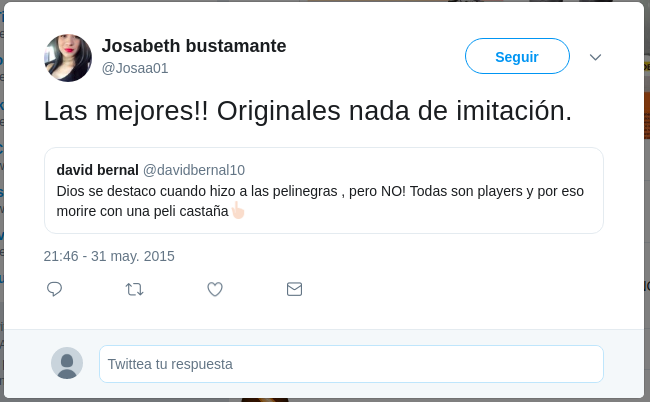
\includegraphics[width=\linewidth]{imagenes/ejemploTweet.png}
	\caption{Ejemplo real de tweet.}
	\label{fig:ejTweet}
\end{figure}

\par Se extrae el texto y se ve en el corpus como lo siguiente texto:

\begin{center}
	605233873635508224|0|Las mejores!! Originales nada de imitación. http://link \\[6pt]
	\footnotesize{Extracción de únicamente texto.}
\end{center}

\par Como se ve en este texto, el primer elemento es el número de identificación del tweet, el cual en combinación con el id de usuario se puede obtener la liga al tweet.

\vspace{5pt}
\begin{center}
	\par https://twitter.com/Josaa01/status/605233873635508224
\end{center}

\vspace{5pt}
\par Luego, el siguiente número simboliza si el texto es irónico o no, un 0 para no irónico y un 1 para un irónico, y por último el texto del tweet.

\par Para la generación de este corpus se consideró que el sarcasmo es un subconjunto de la ironía y se confía absolutamente en la etiqueta que los usuarios proporcionan, aún cuando ésta no sea totalmente fiel a la definición de ironía, cualquiera que quiera considerarse. Pero el corpus de esta tesis no es el mismo que el que usaron \textcite{lopez2016character}, ya que después de que ellos lo usaron, el corpus se sometió a un etiquetado manual. La distribución del corpus es la sugerida en el mismo texto, 90\% no irónicos y 10\% irónicos, lo cual ya no los hace directamente comparables.

\par De este modo, se puede ver desde un principio que la definición que se busca es lo que convencionalmente se considera como ironía y no la definición rigurosa de ésta, por lo que a pesar de tratar de atajar una característica general del lenguaje, esta solución está limitada a las condiciones para las que fue entrenada, es decir, para Twitter en idioma español y lo que las personas que etiquetaron manualmente el corpus consideraron como irónico.

\par El corpus se obtuvo mediante la API que Twitter provee para el lenguaje Ruby. Esto diferencia el presente trabajo de algunos otros de la bibliografía. Para obtener los tweets que se usan como fondo, es decir, muestras no relevantes para la clase irónica, se buscarón diferentes palabras con un significado vacío, el cual se proponía no sesgar la búsqueda a un tema específico; estas palabras fueron: donde, quien, como, cuando, este, tiene, porque, dónde, quién, cómo, cuándo, esta, está y por qué. Para obtener los tweets con carácter irónico o sarcástico se uso la búsqueda de \textit{ \#sarcasmo} y \textit{\#ironía}. Adicional a esto se hizo una verificación manual de los tweets que son irónicos y los que no. Se omitieron las referencias a usuarios remplazando el \textit{@user} por \textit{@} y las ligas por \textit{http://link}.

\par Este es el primer estudio que se hace con el corpus etiquetado manualmente, lo que lo diferencia de la gran mayoría de los de la bibliografía, que confiaban que fueran los autores de las sentencias los que etiquetaran correctamente las oraciones. Esto tiene dos puntos de vista: por un lado con el etiquetado manual, no se encuentra una universalidad de lo que es una sentencia irónica, sino que se entrena al sistema a reconocer las oraciones irónicas que una persona reconoce como tal. Por otro lado, si no se etiqueta manualmente, no se tiene un mismo criterio para clasificar a las oraciones, éstas podrían resultar muchas veces contradictorias, por que donde uno ve ironía otro ve enojo, tristeza, etc.

\section{Preprocesamiento}

\par Una vez obtenido el corpus, el primer paso que se debe llevar a cabo es la interpretación del texto crudo a un dominio que la computadora pueda manejar correctamente; con esta intención existen muchos enfoques, como se vio en el capítulo \ref{cap.introduccion} y en este estudio se uso el que se presenta a continuación.
\subsection{Proceso de preprocesamiento}
\par Con el objetivo de convertir las cadenas de texto en objetos que la computadora pueda manejar fácilmente, se propuso usar una función hash que trabaja como diccionario para las palabras que se han visto en el corpus\footnote{Más concretamente en el subconjunto de entrenamiento.}.
\begin{figure}[h]
	\centering
	

\tikzset{every picture/.style={line width=0.75pt}} %set default line width to 0.75pt        

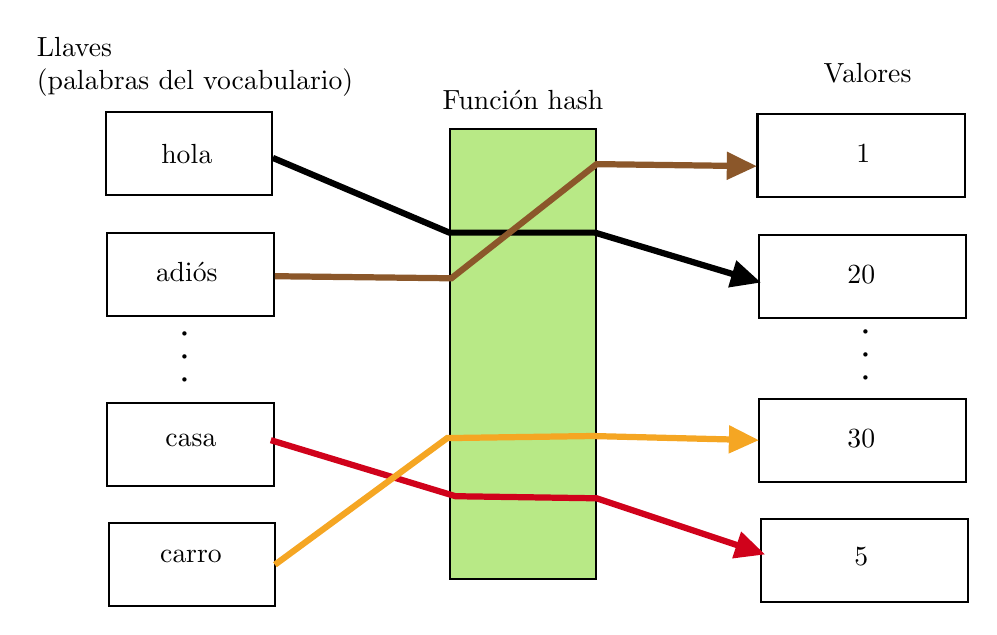
\begin{tikzpicture}[x=0.75pt,y=0.75pt,yscale=-1,xscale=1]
%uncomment if require: \path (0,334); %set diagram left start at 0, and has height of 334

%Shape: Rectangle [id:dp9405282177144714] 
\draw  [fill={rgb, 255:red, 184; green, 233; blue, 134 }  ,fill opacity=1 ] (253,50) -- (323,50) -- (323,267) -- (253,267) -- cycle ;
%Shape: Rectangle [id:dp8774923706333706] 
\draw   (401,43) -- (500.84,43) -- (500.84,83) -- (401,83) -- cycle ;
%Shape: Rectangle [id:dp09572839834830282] 
\draw   (401.83,101) -- (501.67,101) -- (501.67,141) -- (401.83,141) -- cycle ;
%Shape: Rectangle [id:dp1880999561103287] 
\draw   (401.83,180) -- (501.67,180) -- (501.67,220) -- (401.83,220) -- cycle ;
%Shape: Rectangle [id:dp4928306397366884] 
\draw   (402.66,238) -- (502.5,238) -- (502.5,278) -- (402.66,278) -- cycle ;
%Shape: Rectangle [id:dp06784076437826858] 
\draw   (87,42) -- (167.17,42) -- (167.17,82) -- (87,82) -- cycle ;
%Shape: Rectangle [id:dp9784309669414966] 
\draw   (87.67,100) -- (167.83,100) -- (167.83,140) -- (87.67,140) -- cycle ;
%Shape: Rectangle [id:dp34939452369495627] 
\draw   (87.67,182) -- (167.83,182) -- (167.83,222) -- (87.67,222) -- cycle ;
%Shape: Rectangle [id:dp41241321461007474] 
\draw   (88.33,240) -- (168.5,240) -- (168.5,280) -- (88.33,280) -- cycle ;
%Straight Lines [id:da9671353619044671] 
\draw [line width=2.25]    (167.5,64) -- (252.5,100) -- (322.68,100) -- (398.67,122.85) ;
\draw [shift={(402.5,124)}, rotate = 196.73] [fill={rgb, 255:red, 0; green, 0; blue, 0 }  ][line width=2.25]  [draw opacity=0] (14.29,-6.86) -- (0,0) -- (14.29,6.86) -- cycle    ;

%Straight Lines [id:da5193499988670736] 
\draw [color={rgb, 255:red, 139; green, 87; blue, 42 }  ,draw opacity=1 ][line width=2.25]    (168.5,121) -- (253.5,122) -- (323.5,67) -- (396.5,67.95) ;
\draw [shift={(400.5,68)}, rotate = 180.74] [fill={rgb, 255:red, 139; green, 87; blue, 42 }  ,fill opacity=1 ][line width=2.25]  [draw opacity=0] (14.29,-6.86) -- (0,0) -- (14.29,6.86) -- cycle    ;

%Straight Lines [id:da4044543016300448] 
\draw [color={rgb, 255:red, 208; green, 2; blue, 27 }  ,draw opacity=1 ][line width=2.25]    (166.5,200) -- (255.5,227) -- (323.5,228) -- (400.71,253.74) ;
\draw [shift={(404.5,255)}, rotate = 198.43] [fill={rgb, 255:red, 208; green, 2; blue, 27 }  ,fill opacity=1 ][line width=2.25]  [draw opacity=0] (14.29,-6.86) -- (0,0) -- (14.29,6.86) -- cycle    ;

%Straight Lines [id:da9966552915826332] 
\draw [color={rgb, 255:red, 245; green, 166; blue, 35 }  ,draw opacity=1 ][line width=2.25]    (168.5,260) -- (251.5,199) -- (321.5,198) -- (397.5,199.9) ;
\draw [shift={(401.5,200)}, rotate = 181.43] [fill={rgb, 255:red, 245; green, 166; blue, 35 }  ,fill opacity=1 ][line width=2.25]  [draw opacity=0] (14.29,-6.86) -- (0,0) -- (14.29,6.86) -- cycle    ;


% Text Node
\draw (288,36) node  [align=left] {Función hash};
% Text Node
\draw (130,20) node  [align=left] {		Llaves \\(palabras del vocabulario)};
% Text Node
\draw (454,23) node  [align=left] {Valores};
% Text Node
\draw (126,62) node  [align=left] {hola};
% Text Node
\draw (126,119) node  [align=left] {adiós};
% Text Node
\draw (128,200) node  [align=left] {casa};
% Text Node
\draw (128,256) node  [align=left] {carro};
% Text Node
\draw (452,62) node  [align=left] {1};
% Text Node
\draw (451,120) node  [align=left] {20};
% Text Node
\draw (451,199) node  [align=left] {30};
% Text Node
\draw (451,256) node  [align=left] {5};
% Text Node
\draw (125,160) node [rotate=-90] [align=left] {\textbf{. . .}};
% Text Node
\draw (453,159) node [rotate=-90] [align=left] {\textbf{. . .}};


\end{tikzpicture}

	\caption{Funcionamiento de una función hash.}
	\label{fig:funcionHash}
\end{figure}
\par Tal como se ve en la figura \ref{fig:funcionHash}, la función que mapea las palabras a objetos (en este caso se usarán números enteros por simplicidad) es una función hash, la cual necesitará, primero, un conjunto de palabras que conforman los tweets. Dichas palabras\footnote{Considérese
	una palabra una subcadena que separa de otras por un espacio, coma o punto.} deberán aparecer al menos 5 veces\footnote{Este valor se fijó experimentalmente, ya que no se ignoraban tantas y filtraba las palabras que menos se mencionaban.}. Si la palabra no alcanza ese número de apariciones, se considera como \textit{UNK} que significa \textit{unknown} o desconocida, lo cual simboliza que existe un pedazo de información que falta o que tiene un significado desconocido. En este proceso que crea el vocabulario, no se ignoraron palabras que generalmente no aportan información valiosa para la clasificación, tales como: de, y, a, o, del, el, entre otras.

\par Otro enfoque es considerar como unidad de información los carácteres que conforman la oración. Esto aporta información diferente, ya que en lugar de omitir datos que pueden ser considerados basura, se incluyen todos los datos y se permite que el modelo decida si son útiles o no. Para esto puede aumentarse el tamaño de la unidad mínima, desde un carácter hasta n; este método se le conoce como n-gramas o \textit{n-grams} en inglés.

\subsection{Diferentes enfoques en el preprocesamiento}

\par Desde la perspectiva de otros investigadores, fue más importante considerar un conjunto de reglas que modelara estrictamente lo que es la ironía, como se vio con \textcite{utsumi1996unified} y \textcite{kong2011formalization}, lo cual se puede considerar como una buena solución si se desea conocer mejor el lenguaje propio para el cual se  hace el modelo, pero ineficiente y poco adaptable a los casos de la vida real dónde el lenguaje está vivo y cambia mucho dependiendo del contexto y del uso de las palabras. Este estudio tiene esta ventaja ya que va a adaptarse a lo que algunos usuarios de esta red social han considerado como ironía o no.

\par Por otro lado, algunos investigadores consideraron usar etiquetas \gls{POS} las cuales dan a las palabras características únicas como la de ser un verbo, adjetivo, adverbio, sustantivo, entre otras. Estas características resultan importantes para obtener las fórmulas que describirían un texto sarcástico o irónico, como lo hizo \textcite{barbieri2014italian} y similar a los que hizo \textcite{davidov2010semi}. Sin embargo, con este acercamiento hay ciertas precauciones, ya que es necesario saber cómo se usa cierta palabra en un momento dado y vienen a la luz dos tipos de problemas. El primero corresponde al uso indistinto de algunas palabras como \textit{`vino'}, cuando se usa como verbo y cuando se usa como sustantivo. Este problema podría manejarse tal vez adaptando el árbol de decisiones que se usó en \textcite{barbieri2014italian} para que regrese las diferentes variantes que podría dar como resultado que se considere como verbo o como sustantivo. El segundo problema es cuando se deriva un sustantivo en un verbo; en estos casos no podría entenderse qué significado se le puede dar; estos problemas se atajan en la solución debido a que no se da por hecho lo que el usuario quiere decir, con una palabra o qué uso quiere darle.


\subsection{Complejidad del preprocesamiento}

La complejidad de este preprocesamiento es lineal, ya que se debe leer cada palabra de cada tweet dos veces, la primera para obtener las palabras que conforman todo el corpus y contar si esta palabra entrará en el vocabulario, y la segunda para asignarle a cada tweet un vector de índices que corresponden al vocabulario que se obtuvo antes.


\section{Técnica de clasificación - Redes neuronales}

\par La técnica que se consideró para este problema fue una red neuronal con arquitectura \gls{bi-lstm} la cual le permite formar un resumen de lo que existe delante de su punto de estudio actual y antes de ese punto. La \gls{bi-lstm} se usa en análisis de textos ampliamente, debido a que los textos tienen esta estructura lineal. A continuación se explicará detalladamente en qué consiste una red neuronal y posteriormente se describirá el funcionamiento de un \gls{bi-lstm}.

\par En el área de la inteligencia artificial existe una técnica de clasificación inspirada en el funcionamiento del cerebro, para el cual primero se modela la función de una neurona como elemento básico. Este modelo fue primero elaborado en 1943 por \textcite{mcculloch1943logical} en la que modelaba matemáticamente el funcionamiento de una neurona. El enfoque que ellos tomaban era considerar que las neuronas podían tratarse con lógica proposicional, la cual ha ido evolucionando a través de los años.  \textcite{rosenblatt1958perceptron} propuso el modelo de un perceptrón simple basado en las ideas de \textcite{mcculloch1943logical}; la teoría de Rosenblatt se basaba más en un acercamiento probabilístico del funcionamiento de las neuronas en lugar del booleano de McCulloch. Este modelo es un perceptrón de dos capas, la de entrada y la de salida.

\subsection{Funcionamiento}

\par Este modelo se puede definir como un sistema con entradas y salidas las cuales pasan por una unidad sumadora que las compara con un umbral (\textit{bias} en inglés), la cual activa una función de salida no lineal. Su funcionamiento es simple, y se puede notar que lo que propone es que la salida de un sistema que se puede clasificar es el resultado de la combinación lineal de las entradas con un valor de desplazamiento a la salida(\textit{bias}). Luego, la función de salida podría interpretarse como booleana, un 1 si alcanzó el valor de umbral $\theta_{0}$ o un 0 si no. Lo anterior puede interpretarse como que todo lo que esté debajo de una recta definida por $(\theta_0,\theta_1,...,\theta_n)$ se considera que no pertenece a la clase y lo que está por encima de ella pertenece a dicha clase. En la figura \ref{fig:perceptron} se puede ver el funcionamiento de una sola neurona.
\begin{figure}[H]
	\centering
	

\tikzset{every picture/.style={line width=0.75pt}} %set default line width to 0.75pt        

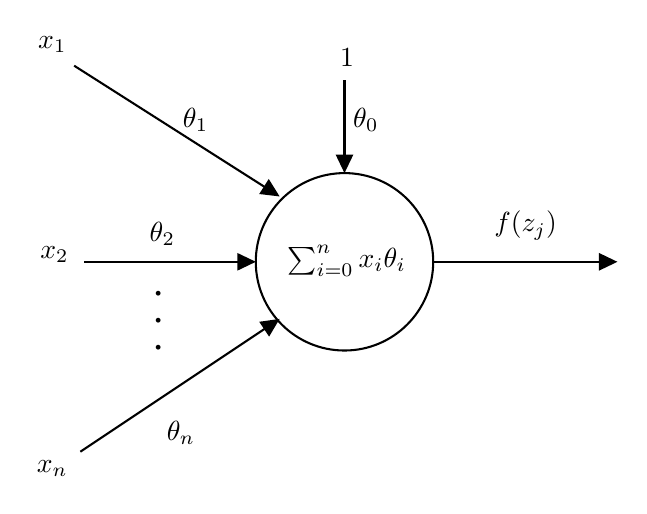
\begin{tikzpicture}[x=0.75pt,y=0.75pt,yscale=-1,xscale=1]
%uncomment if require: \path (0,300); %set diagram left start at 0, and has height of 300

%Straight Lines [id:da680897344066558] 
\draw    (223.5,117.49) -- (310.25,117.49) ;
\draw [shift={(312.25,117.49)}, rotate = 180] [fill={rgb, 255:red, 0; green, 0; blue, 0 }  ][line width=0.75]  [draw opacity=0] (8.93,-4.29) -- (0,0) -- (8.93,4.29) -- cycle    ;

%Shape: Circle [id:dp9729890208928396] 
\draw   (138.02,117.49) .. controls (138.02,93.89) and (157.15,74.75) .. (180.76,74.75) .. controls (204.36,74.75) and (223.5,93.89) .. (223.5,117.49) .. controls (223.5,141.1) and (204.36,160.23) .. (180.76,160.23) .. controls (157.15,160.23) and (138.02,141.1) .. (138.02,117.49) -- cycle ;
%Straight Lines [id:da595997026089699] 
\draw    (50.5,23) -- (147.81,84.93) ;
\draw [shift={(149.5,86)}, rotate = 212.47] [fill={rgb, 255:red, 0; green, 0; blue, 0 }  ][line width=0.75]  [draw opacity=0] (8.93,-4.29) -- (0,0) -- (8.93,4.29) -- cycle    ;

%Straight Lines [id:da17014503403275416] 
\draw    (55.49,117.49) -- (136.02,117.49) ;
\draw [shift={(138.02,117.49)}, rotate = 540] [fill={rgb, 255:red, 0; green, 0; blue, 0 }  ][line width=0.75]  [draw opacity=0] (8.93,-4.29) -- (0,0) -- (8.93,4.29) -- cycle    ;

%Straight Lines [id:da3776987769018221] 
\draw    (53.5,209) -- (147.84,146.11) ;
\draw [shift={(149.5,145)}, rotate = 506.31] [fill={rgb, 255:red, 0; green, 0; blue, 0 }  ][line width=0.75]  [draw opacity=0] (8.93,-4.29) -- (0,0) -- (8.93,4.29) -- cycle    ;

%Straight Lines [id:da22738163646288978] 
\draw    (180.76,30.12) -- (180.76,72.75) ;
\draw [shift={(180.76,74.75)}, rotate = 270] [fill={rgb, 255:red, 0; green, 0; blue, 0 }  ][line width=0.75]  [draw opacity=0] (8.93,-4.29) -- (0,0) -- (8.93,4.29) -- cycle    ;


% Text Node
\draw (184,117) node   {$\sum ^{n}_{i=0} x_{i} \theta _{i} \ $};
% Text Node
\draw (91,146) node [rotate=-90] [align=left] {\textbf{{\large . . .}}};
% Text Node
\draw (40,13) node   {$x_{1}$};
% Text Node
\draw (41,114) node   {$x_{2}$};
% Text Node
\draw (40,217) node   {$x_{n}$};
% Text Node
\draw (182,19) node   {$1$};
% Text Node
\draw (109,49) node   {$\theta _{1}$};
% Text Node
\draw (93,104) node   {$\theta _{2}$};
% Text Node
\draw (102,200) node   {$\theta _{n}$};
% Text Node
\draw (268,100) node   {$f( z_{j})$};
% Text Node
\draw (191,49) node   {$\theta _{0}$};


\end{tikzpicture}

	\caption{Concepto básico del perceptrón simple. Se puede notar que la neurona se activa cuando la combinación lineal de sus entradas producen un resultado mayor al que se tiene como umbral.}
	\label{fig:perceptron}
\end{figure}

\par Tiempo después se demostró que no podía resolver problemas no lineales, con una sola capa del perceptrón, como la compuerta lógica XOR.
\begin{figure}[H]
	\begin{minipage}{0.5\textwidth}
		
\begin{tabular}{|p{0.23093\textwidth}|p{0.23093\textwidth}|p{0.23505\textwidth}|}
\hline
\small{Entrada\ A} & \small{Entrada\ B} & \small{Salida}\\
\hline
\small{0} & \small{0} & \small{0}\\
\hline
\small{0} & \small{1} & \small{1}\\
\hline
\small{1} & \small{0} & \small{1}\\
\hline
\small{1} & \small{1} & \small{0}\\
\hline
\end{tabular}

	\end{minipage}%
	\begin{minipage}{0.5\textwidth}
		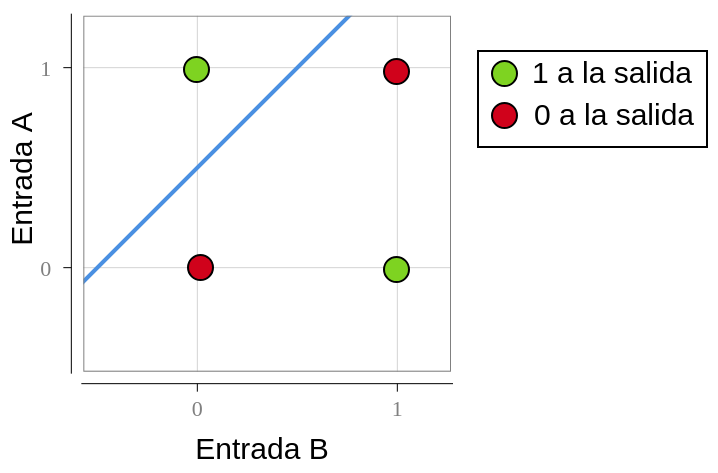
\includegraphics[width=\textwidth]{imagenes/diagramaXor.png}
	\end{minipage}
	\caption{No es posible separar con una capa de perceptrón la salida de una compuerta XOR.}
	\label{fig:xor}
\end{figure}


\par Como se ve en la figura \ref{fig:xor} para poder resolver este tipo de problemas se propuso usar más capas del perceptrón que podrían resolver el problema fácilmente, ya que cuando se agregan más perceptrones, se pueden \textit{`dibujar'} más lineas que puedan ayudar a dividir mejor una clase. Como se puede ver en la figura \ref{fig:xor2}.

\begin{figure}[H]
	\centering
	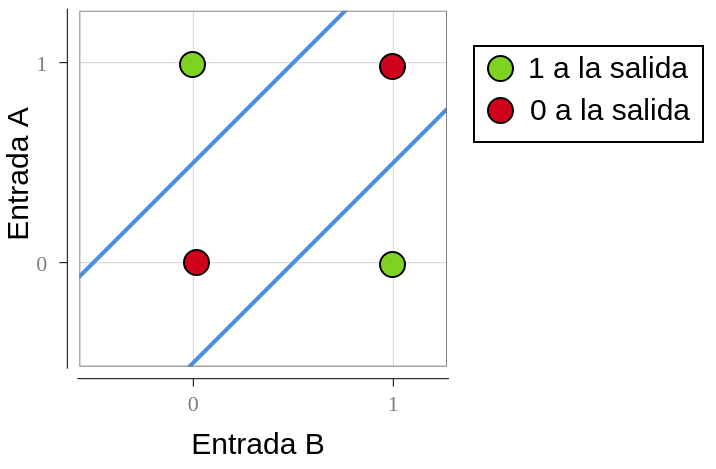
\includegraphics[width=0.5\textwidth]{imagenes/diagramaXor2.png}
	\caption{Usando una capa más se puede dividir la salida de la compuerta XOR.}
	\label{fig:xor2}
\end{figure}

\par Una red neuronal se entiende comunmente como un conjunto de perceptrones interconectados que hacen aún más compleja la salida de un simple perceptrón. Además, se le conoce con varios nombres en los textos científicos como son \textit{red neuronal completamente conectada}, \textit{\gls{mlp}} y \textit{densa}. Para el caso de cada perceptrón, deberán aplicarse las mismas operaciones que se habían descrito. 
\par Esta consta de tres partes esenciales: 
	\begin{itemize}
		\item capa de entrada, la cual se encarga únicamente de recibir los datos, procesarlos y pasarlos a la capa oculta;
		\item capa oculta, la cual constituye la mayor parte del procesamiento, aquí se extraen más características y se pasan a la capa de salida;
		\item  capa de salida, esta capa puede tener una o más salidas, las cuales pueden simbolizar las clases que se desean discriminar.
	\end{itemize}

\par En la figura \ref{fig:redneuronal1} se puede observar cómo se calcula la salida de la primera neurona de la primera capa.

\begin{figure}[h]
	\centering
	

\tikzset{every picture/.style={line width=0.75pt}} %set default line width to 0.75pt        

\begin{tikzpicture}[x=0.75pt,y=0.75pt,yscale=-1,xscale=1]
%uncomment if require: \path (0,320); %set diagram left start at 0, and has height of 320

%Straight Lines [id:da8798173448108342] 
\draw [color={rgb, 255:red, 155; green, 155; blue, 155 }  ,draw opacity=1 ]   (93.5,67.25) -- (130.19,150.42) ;
\draw [shift={(131,152.25)}, rotate = 246.19] [fill={rgb, 255:red, 155; green, 155; blue, 155 }  ,fill opacity=1 ][line width=0.75]  [draw opacity=0] (8.93,-4.29) -- (0,0) -- (8.93,4.29) -- cycle    ;

%Straight Lines [id:da1264938029525713] 
\draw [color={rgb, 255:red, 155; green, 155; blue, 155 }  ,draw opacity=1 ]   (93.5,67.25) -- (132.57,243.3) ;
\draw [shift={(133,245.25)}, rotate = 257.49] [fill={rgb, 255:red, 155; green, 155; blue, 155 }  ,fill opacity=1 ][line width=0.75]  [draw opacity=0] (8.93,-4.29) -- (0,0) -- (8.93,4.29) -- cycle    ;

%Straight Lines [id:da4251940989802534] 
\draw [color={rgb, 255:red, 155; green, 155; blue, 155 }  ,draw opacity=1 ]   (93.5,116.25) -- (129.56,150.86) ;
\draw [shift={(131,152.25)}, rotate = 223.82999999999998] [fill={rgb, 255:red, 155; green, 155; blue, 155 }  ,fill opacity=1 ][line width=0.75]  [draw opacity=0] (8.93,-4.29) -- (0,0) -- (8.93,4.29) -- cycle    ;

%Straight Lines [id:da608901596398933] 
\draw [color={rgb, 255:red, 155; green, 155; blue, 155 }  ,draw opacity=1 ]   (93.5,116.25) -- (132.41,243.34) ;
\draw [shift={(133,245.25)}, rotate = 252.98000000000002] [fill={rgb, 255:red, 155; green, 155; blue, 155 }  ,fill opacity=1 ][line width=0.75]  [draw opacity=0] (8.93,-4.29) -- (0,0) -- (8.93,4.29) -- cycle    ;

%Straight Lines [id:da22280654479157525] 
\draw [color={rgb, 255:red, 155; green, 155; blue, 155 }  ,draw opacity=1 ]   (94.5,163.25) -- (129.09,152.83) ;
\draw [shift={(131,152.25)}, rotate = 523.23] [fill={rgb, 255:red, 155; green, 155; blue, 155 }  ,fill opacity=1 ][line width=0.75]  [draw opacity=0] (8.93,-4.29) -- (0,0) -- (8.93,4.29) -- cycle    ;

%Straight Lines [id:da6030354960312154] 
\draw [color={rgb, 255:red, 155; green, 155; blue, 155 }  ,draw opacity=1 ]   (94.5,163.25) -- (132.15,243.44) ;
\draw [shift={(133,245.25)}, rotate = 244.85] [fill={rgb, 255:red, 155; green, 155; blue, 155 }  ,fill opacity=1 ][line width=0.75]  [draw opacity=0] (8.93,-4.29) -- (0,0) -- (8.93,4.29) -- cycle    ;

%Straight Lines [id:da21636688103646295] 
\draw [color={rgb, 255:red, 155; green, 155; blue, 155 }  ,draw opacity=1 ]   (95.5,236.25) -- (130.22,154.09) ;
\draw [shift={(131,152.25)}, rotate = 472.91] [fill={rgb, 255:red, 155; green, 155; blue, 155 }  ,fill opacity=1 ][line width=0.75]  [draw opacity=0] (8.93,-4.29) -- (0,0) -- (8.93,4.29) -- cycle    ;

%Straight Lines [id:da5980881110108045] 
\draw [color={rgb, 255:red, 155; green, 155; blue, 155 }  ,draw opacity=1 ]   (95.5,236.25) -- (131.06,244.78) ;
\draw [shift={(133,245.25)}, rotate = 193.5] [fill={rgb, 255:red, 155; green, 155; blue, 155 }  ,fill opacity=1 ][line width=0.75]  [draw opacity=0] (8.93,-4.29) -- (0,0) -- (8.93,4.29) -- cycle    ;

%Straight Lines [id:da3351006204177107] 
\draw [color={rgb, 255:red, 155; green, 155; blue, 155 }  ,draw opacity=1 ]   (248.5,42.25) -- (285.24,62.29) ;
\draw [shift={(287,63.25)}, rotate = 208.61] [fill={rgb, 255:red, 155; green, 155; blue, 155 }  ,fill opacity=1 ][line width=0.75]  [draw opacity=0] (8.93,-4.29) -- (0,0) -- (8.93,4.29) -- cycle    ;

%Straight Lines [id:da6626680795590805] 
\draw [color={rgb, 255:red, 155; green, 155; blue, 155 }  ,draw opacity=1 ]   (248.5,42.25) -- (285.07,111.48) ;
\draw [shift={(286,113.25)}, rotate = 242.16] [fill={rgb, 255:red, 155; green, 155; blue, 155 }  ,fill opacity=1 ][line width=0.75]  [draw opacity=0] (8.93,-4.29) -- (0,0) -- (8.93,4.29) -- cycle    ;

%Straight Lines [id:da7726736210859901] 
\draw [color={rgb, 255:red, 155; green, 155; blue, 155 }  ,draw opacity=1 ]   (248.5,42.25) -- (286.38,158.35) ;
\draw [shift={(287,160.25)}, rotate = 251.93] [fill={rgb, 255:red, 155; green, 155; blue, 155 }  ,fill opacity=1 ][line width=0.75]  [draw opacity=0] (8.93,-4.29) -- (0,0) -- (8.93,4.29) -- cycle    ;

%Straight Lines [id:da6779074339555233] 
\draw [color={rgb, 255:red, 155; green, 155; blue, 155 }  ,draw opacity=1 ]   (248.5,42.25) -- (287.59,231.29) ;
\draw [shift={(288,233.25)}, rotate = 258.32] [fill={rgb, 255:red, 155; green, 155; blue, 155 }  ,fill opacity=1 ][line width=0.75]  [draw opacity=0] (8.93,-4.29) -- (0,0) -- (8.93,4.29) -- cycle    ;

%Straight Lines [id:da22497111902415767] 
\draw [color={rgb, 255:red, 155; green, 155; blue, 155 }  ,draw opacity=1 ]   (247.5,97.25) -- (285.48,64.55) ;
\draw [shift={(287,63.25)}, rotate = 499.28] [fill={rgb, 255:red, 155; green, 155; blue, 155 }  ,fill opacity=1 ][line width=0.75]  [draw opacity=0] (8.93,-4.29) -- (0,0) -- (8.93,4.29) -- cycle    ;

%Straight Lines [id:da7915744230148478] 
\draw [color={rgb, 255:red, 155; green, 155; blue, 155 }  ,draw opacity=1 ]   (247.5,97.25) -- (284.15,112.48) ;
\draw [shift={(286,113.25)}, rotate = 202.57] [fill={rgb, 255:red, 155; green, 155; blue, 155 }  ,fill opacity=1 ][line width=0.75]  [draw opacity=0] (8.93,-4.29) -- (0,0) -- (8.93,4.29) -- cycle    ;

%Straight Lines [id:da8444489661109031] 
\draw [color={rgb, 255:red, 155; green, 155; blue, 155 }  ,draw opacity=1 ]   (247.5,97.25) -- (287.43,231.33) ;
\draw [shift={(288,233.25)}, rotate = 253.42000000000002] [fill={rgb, 255:red, 155; green, 155; blue, 155 }  ,fill opacity=1 ][line width=0.75]  [draw opacity=0] (8.93,-4.29) -- (0,0) -- (8.93,4.29) -- cycle    ;

%Straight Lines [id:da180467501143327] 
\draw [color={rgb, 255:red, 155; green, 155; blue, 155 }  ,draw opacity=1 ]   (247.5,152.25) -- (286.19,65.08) ;
\draw [shift={(287,63.25)}, rotate = 473.93] [fill={rgb, 255:red, 155; green, 155; blue, 155 }  ,fill opacity=1 ][line width=0.75]  [draw opacity=0] (8.93,-4.29) -- (0,0) -- (8.93,4.29) -- cycle    ;

%Straight Lines [id:da7179418865674392] 
\draw [color={rgb, 255:red, 155; green, 155; blue, 155 }  ,draw opacity=1 ]   (247.5,152.25) -- (284.59,114.67) ;
\draw [shift={(286,113.25)}, rotate = 494.63] [fill={rgb, 255:red, 155; green, 155; blue, 155 }  ,fill opacity=1 ][line width=0.75]  [draw opacity=0] (8.93,-4.29) -- (0,0) -- (8.93,4.29) -- cycle    ;

%Straight Lines [id:da35423297686642163] 
\draw [color={rgb, 255:red, 155; green, 155; blue, 155 }  ,draw opacity=1 ]   (247.5,152.25) -- (285.04,159.85) ;
\draw [shift={(287,160.25)}, rotate = 191.45] [fill={rgb, 255:red, 155; green, 155; blue, 155 }  ,fill opacity=1 ][line width=0.75]  [draw opacity=0] (8.93,-4.29) -- (0,0) -- (8.93,4.29) -- cycle    ;

%Straight Lines [id:da8222185311967365] 
\draw [color={rgb, 255:red, 155; green, 155; blue, 155 }  ,draw opacity=1 ]   (247.5,152.25) -- (287.11,231.46) ;
\draw [shift={(288,233.25)}, rotate = 243.43] [fill={rgb, 255:red, 155; green, 155; blue, 155 }  ,fill opacity=1 ][line width=0.75]  [draw opacity=0] (8.93,-4.29) -- (0,0) -- (8.93,4.29) -- cycle    ;

%Straight Lines [id:da6366233578085132] 
\draw [color={rgb, 255:red, 155; green, 155; blue, 155 }  ,draw opacity=1 ]   (249.5,245.25) -- (286.6,65.21) ;
\draw [shift={(287,63.25)}, rotate = 461.64] [fill={rgb, 255:red, 155; green, 155; blue, 155 }  ,fill opacity=1 ][line width=0.75]  [draw opacity=0] (8.93,-4.29) -- (0,0) -- (8.93,4.29) -- cycle    ;

%Straight Lines [id:da19092990208654426] 
\draw [color={rgb, 255:red, 155; green, 155; blue, 155 }  ,draw opacity=1 ]   (249.5,245.25) -- (285.47,115.18) ;
\draw [shift={(286,113.25)}, rotate = 465.46] [fill={rgb, 255:red, 155; green, 155; blue, 155 }  ,fill opacity=1 ][line width=0.75]  [draw opacity=0] (8.93,-4.29) -- (0,0) -- (8.93,4.29) -- cycle    ;

%Straight Lines [id:da5250825232708285] 
\draw [color={rgb, 255:red, 155; green, 155; blue, 155 }  ,draw opacity=1 ]   (249.5,245.25) -- (286.19,162.08) ;
\draw [shift={(287,160.25)}, rotate = 473.81] [fill={rgb, 255:red, 155; green, 155; blue, 155 }  ,fill opacity=1 ][line width=0.75]  [draw opacity=0] (8.93,-4.29) -- (0,0) -- (8.93,4.29) -- cycle    ;

%Straight Lines [id:da06185650174435953] 
\draw [color={rgb, 255:red, 155; green, 155; blue, 155 }  ,draw opacity=1 ]   (249.5,245.25) -- (286.09,233.85) ;
\draw [shift={(288,233.25)}, rotate = 522.69] [fill={rgb, 255:red, 155; green, 155; blue, 155 }  ,fill opacity=1 ][line width=0.75]  [draw opacity=0] (8.93,-4.29) -- (0,0) -- (8.93,4.29) -- cycle    ;

%Shape: Circle [id:dp8378261731976331] 
\draw   (60,66.25) .. controls (60,56.72) and (67.72,49) .. (77.25,49) .. controls (86.78,49) and (94.5,56.72) .. (94.5,66.25) .. controls (94.5,75.78) and (86.78,83.5) .. (77.25,83.5) .. controls (67.72,83.5) and (60,75.78) .. (60,66.25) -- cycle ;
%Shape: Circle [id:dp6886548408081758] 
\draw   (61,236.25) .. controls (61,226.72) and (68.72,219) .. (78.25,219) .. controls (87.78,219) and (95.5,226.72) .. (95.5,236.25) .. controls (95.5,245.78) and (87.78,253.5) .. (78.25,253.5) .. controls (68.72,253.5) and (61,245.78) .. (61,236.25) -- cycle ;
%Shape: Circle [id:dp46631909550454664] 
\draw   (59,116.25) .. controls (59,106.72) and (66.72,99) .. (76.25,99) .. controls (85.78,99) and (93.5,106.72) .. (93.5,116.25) .. controls (93.5,125.78) and (85.78,133.5) .. (76.25,133.5) .. controls (66.72,133.5) and (59,125.78) .. (59,116.25) -- cycle ;
%Shape: Circle [id:dp624774125190017] 
\draw   (60,163.25) .. controls (60,153.72) and (67.72,146) .. (77.25,146) .. controls (86.78,146) and (94.5,153.72) .. (94.5,163.25) .. controls (94.5,172.78) and (86.78,180.5) .. (77.25,180.5) .. controls (67.72,180.5) and (60,172.78) .. (60,163.25) -- cycle ;
%Straight Lines [id:da4326296089497377] 
\draw    (41.02,66.25) -- (58,66.25) ;
\draw [shift={(60,66.25)}, rotate = 180] [fill={rgb, 255:red, 0; green, 0; blue, 0 }  ][line width=0.75]  [draw opacity=0] (8.93,-4.29) -- (0,0) -- (8.93,4.29) -- cycle    ;

%Straight Lines [id:da7377396516203609] 
\draw    (40.02,116.25) -- (57,116.25) ;
\draw [shift={(59,116.25)}, rotate = 180] [fill={rgb, 255:red, 0; green, 0; blue, 0 }  ][line width=0.75]  [draw opacity=0] (8.93,-4.29) -- (0,0) -- (8.93,4.29) -- cycle    ;

%Straight Lines [id:da772460813491475] 
\draw    (41.02,163.25) -- (58,163.25) ;
\draw [shift={(60,163.25)}, rotate = 180] [fill={rgb, 255:red, 0; green, 0; blue, 0 }  ][line width=0.75]  [draw opacity=0] (8.93,-4.29) -- (0,0) -- (8.93,4.29) -- cycle    ;

%Straight Lines [id:da9681905997792641] 
\draw    (42.02,236.25) -- (59,236.25) ;
\draw [shift={(61,236.25)}, rotate = 180] [fill={rgb, 255:red, 0; green, 0; blue, 0 }  ][line width=0.75]  [draw opacity=0] (8.93,-4.29) -- (0,0) -- (8.93,4.29) -- cycle    ;

%Shape: Circle [id:dp21825918883593576] 
\draw   (132,42.25) .. controls (132,32.72) and (139.72,25) .. (149.25,25) .. controls (158.78,25) and (166.5,32.72) .. (166.5,42.25) .. controls (166.5,51.78) and (158.78,59.5) .. (149.25,59.5) .. controls (139.72,59.5) and (132,51.78) .. (132,42.25) -- cycle ;
%Shape: Circle [id:dp547845684421643] 
\draw   (133,245.25) .. controls (133,235.72) and (140.72,228) .. (150.25,228) .. controls (159.78,228) and (167.5,235.72) .. (167.5,245.25) .. controls (167.5,254.78) and (159.78,262.5) .. (150.25,262.5) .. controls (140.72,262.5) and (133,254.78) .. (133,245.25) -- cycle ;
%Shape: Circle [id:dp8711680643696975] 
\draw   (131,97.25) .. controls (131,87.72) and (138.72,80) .. (148.25,80) .. controls (157.78,80) and (165.5,87.72) .. (165.5,97.25) .. controls (165.5,106.78) and (157.78,114.5) .. (148.25,114.5) .. controls (138.72,114.5) and (131,106.78) .. (131,97.25) -- cycle ;
%Shape: Circle [id:dp8241885312698898] 
\draw   (131,152.25) .. controls (131,142.72) and (138.72,135) .. (148.25,135) .. controls (157.78,135) and (165.5,142.72) .. (165.5,152.25) .. controls (165.5,161.78) and (157.78,169.5) .. (148.25,169.5) .. controls (138.72,169.5) and (131,161.78) .. (131,152.25) -- cycle ;
%Shape: Circle [id:dp7119276185561412] 
\draw   (214,42.25) .. controls (214,32.72) and (221.72,25) .. (231.25,25) .. controls (240.78,25) and (248.5,32.72) .. (248.5,42.25) .. controls (248.5,51.78) and (240.78,59.5) .. (231.25,59.5) .. controls (221.72,59.5) and (214,51.78) .. (214,42.25) -- cycle ;
%Shape: Circle [id:dp3179021384105416] 
\draw   (215,245.25) .. controls (215,235.72) and (222.72,228) .. (232.25,228) .. controls (241.78,228) and (249.5,235.72) .. (249.5,245.25) .. controls (249.5,254.78) and (241.78,262.5) .. (232.25,262.5) .. controls (222.72,262.5) and (215,254.78) .. (215,245.25) -- cycle ;
%Shape: Circle [id:dp8755056890726975] 
\draw   (213,97.25) .. controls (213,87.72) and (220.72,80) .. (230.25,80) .. controls (239.78,80) and (247.5,87.72) .. (247.5,97.25) .. controls (247.5,106.78) and (239.78,114.5) .. (230.25,114.5) .. controls (220.72,114.5) and (213,106.78) .. (213,97.25) -- cycle ;
%Shape: Circle [id:dp4747564535552429] 
\draw   (213,152.25) .. controls (213,142.72) and (220.72,135) .. (230.25,135) .. controls (239.78,135) and (247.5,142.72) .. (247.5,152.25) .. controls (247.5,161.78) and (239.78,169.5) .. (230.25,169.5) .. controls (220.72,169.5) and (213,161.78) .. (213,152.25) -- cycle ;
%Shape: Circle [id:dp8197699354277264] 
\draw   (287,63.25) .. controls (287,53.72) and (294.72,46) .. (304.25,46) .. controls (313.78,46) and (321.5,53.72) .. (321.5,63.25) .. controls (321.5,72.78) and (313.78,80.5) .. (304.25,80.5) .. controls (294.72,80.5) and (287,72.78) .. (287,63.25) -- cycle ;
%Shape: Circle [id:dp8721964334353247] 
\draw   (288,233.25) .. controls (288,223.72) and (295.72,216) .. (305.25,216) .. controls (314.78,216) and (322.5,223.72) .. (322.5,233.25) .. controls (322.5,242.78) and (314.78,250.5) .. (305.25,250.5) .. controls (295.72,250.5) and (288,242.78) .. (288,233.25) -- cycle ;
%Shape: Circle [id:dp5987591258534826] 
\draw   (286,113.25) .. controls (286,103.72) and (293.72,96) .. (303.25,96) .. controls (312.78,96) and (320.5,103.72) .. (320.5,113.25) .. controls (320.5,122.78) and (312.78,130.5) .. (303.25,130.5) .. controls (293.72,130.5) and (286,122.78) .. (286,113.25) -- cycle ;
%Shape: Circle [id:dp49752905656026436] 
\draw   (287,160.25) .. controls (287,150.72) and (294.72,143) .. (304.25,143) .. controls (313.78,143) and (321.5,150.72) .. (321.5,160.25) .. controls (321.5,169.78) and (313.78,177.5) .. (304.25,177.5) .. controls (294.72,177.5) and (287,169.78) .. (287,160.25) -- cycle ;
%Straight Lines [id:da2893286552413561] 
\draw    (322.02,63.25) -- (339,63.25) ;
\draw [shift={(341,63.25)}, rotate = 180] [fill={rgb, 255:red, 0; green, 0; blue, 0 }  ][line width=0.75]  [draw opacity=0] (8.93,-4.29) -- (0,0) -- (8.93,4.29) -- cycle    ;

%Straight Lines [id:da31837181970999007] 
\draw    (321.02,113.25) -- (338,113.25) ;
\draw [shift={(340,113.25)}, rotate = 180] [fill={rgb, 255:red, 0; green, 0; blue, 0 }  ][line width=0.75]  [draw opacity=0] (8.93,-4.29) -- (0,0) -- (8.93,4.29) -- cycle    ;

%Straight Lines [id:da7130677314020706] 
\draw    (322.02,160.25) -- (339,160.25) ;
\draw [shift={(341,160.25)}, rotate = 180] [fill={rgb, 255:red, 0; green, 0; blue, 0 }  ][line width=0.75]  [draw opacity=0] (8.93,-4.29) -- (0,0) -- (8.93,4.29) -- cycle    ;

%Straight Lines [id:da1146408293027561] 
\draw    (323.02,233.25) -- (340,233.25) ;
\draw [shift={(342,233.25)}, rotate = 180] [fill={rgb, 255:red, 0; green, 0; blue, 0 }  ][line width=0.75]  [draw opacity=0] (8.93,-4.29) -- (0,0) -- (8.93,4.29) -- cycle    ;

%Straight Lines [id:da9370970117900812] 
\draw [color={rgb, 255:red, 208; green, 2; blue, 27 }  ,draw opacity=1 ]   (94.5,66.25) -- (129.48,95.96) ;
\draw [shift={(131,97.25)}, rotate = 220.34] [fill={rgb, 255:red, 208; green, 2; blue, 27 }  ,fill opacity=1 ][line width=0.75]  [draw opacity=0] (8.93,-4.29) -- (0,0) -- (8.93,4.29) -- cycle    ;

%Straight Lines [id:da31070588195621585] 
\draw [color={rgb, 255:red, 208; green, 2; blue, 27 }  ,draw opacity=1 ]   (93.5,116.25) -- (129.22,98.15) ;
\draw [shift={(131,97.25)}, rotate = 513.13] [fill={rgb, 255:red, 208; green, 2; blue, 27 }  ,fill opacity=1 ][line width=0.75]  [draw opacity=0] (8.93,-4.29) -- (0,0) -- (8.93,4.29) -- cycle    ;

%Straight Lines [id:da8021804321980563] 
\draw [color={rgb, 255:red, 208; green, 2; blue, 27 }  ,draw opacity=1 ]   (94.5,163.25) -- (130.03,99) ;
\draw [shift={(131,97.25)}, rotate = 478.94] [fill={rgb, 255:red, 208; green, 2; blue, 27 }  ,fill opacity=1 ][line width=0.75]  [draw opacity=0] (8.93,-4.29) -- (0,0) -- (8.93,4.29) -- cycle    ;

%Straight Lines [id:da2185947312717822] 
\draw [color={rgb, 255:red, 208; green, 2; blue, 27 }  ,draw opacity=1 ]   (95.5,236.25) -- (130.51,99.19) ;
\draw [shift={(131,97.25)}, rotate = 464.33] [fill={rgb, 255:red, 208; green, 2; blue, 27 }  ,fill opacity=1 ][line width=0.75]  [draw opacity=0] (8.93,-4.29) -- (0,0) -- (8.93,4.29) -- cycle    ;



% Text Node
\draw (80,201) node [rotate=-90] [align=left] {\textbf{{\large . . .}}};
% Text Node
\draw (152,196) node [rotate=-90] [align=left] {\textbf{{\large . . .}}};
% Text Node
\draw (192,132) node  [align=left] {\textbf{{\large . . .}}};
% Text Node
\draw (234,196) node [rotate=-90] [align=left] {\textbf{{\large . . .}}};
% Text Node
\draw (307,198) node [rotate=-90] [align=left] {\textbf{{\large . . .}}};
% Text Node
\draw (78,66) node   {$1$};
% Text Node
\draw (78,118) node   {$x_{1}$};
% Text Node
\draw (78,163) node   {$x_{2}$};
% Text Node
\draw (79,236) node   {$x_{n}$};
% Text Node
\draw (150,44) node   {$1$};
% Text Node
\draw (149,97) node   {$a^{1}_{1}$};
% Text Node
\draw (149,153) node   {$a^{1}_{2}$};
% Text Node
\draw (151,246) node   {$a^{1}_{m}$};
% Text Node
\draw (232,43) node   {$1$};
% Text Node
\draw (231,97) node   {$a^{k}_{1}$};
% Text Node
\draw (230,151) node   {$a^{k}_{2}$};
% Text Node
\draw (234,244) node   {$a^{k}_{m}$};
% Text Node
\draw (305,63) node   {$y_{1}$};
% Text Node
\draw (304,112) node   {$y_{2}$};
% Text Node
\draw (304,161) node   {$y_{3}$};
% Text Node
\draw (306,232) node   {$y_{l}$};
% Text Node
\draw (111,58) node   {$\theta ^{1}_{01}$};
% Text Node
\draw (105,94) node   {$\theta ^{1}_{11}$};
% Text Node
\draw (102,133) node   {$\theta ^{1}_{21}$};
% Text Node
\draw (117,209) node   {$\theta ^{1}_{n1}$};
% Text Node
\draw (240,283) node   {${\textstyle a^{1}_{1} =f\left( 1\times \theta ^{1}_{01} +x_{1} \times \theta ^{1}_{11} +x_{2} \times \theta ^{1}_{21} +.\ .\ .+x_{n} \times \theta ^{1}_{n1}\right) =f\left( x^{T} \Theta ^{1}_{1}\right)}$};
% Text Node
\draw (445,98) node   {$x=\begin{bmatrix}
1\\
x_{1}\\
x_{2}\\
...\\
x_{n}
\end{bmatrix} \ ;\ \Theta ^{i}_{j} =\begin{bmatrix}
\theta ^{i}_{0}\\
\theta ^{i}_{1}\\
\theta ^{i}_{2}\\
...\\
\theta ^{i}_{n}
\end{bmatrix}$};


\end{tikzpicture}

	\caption{Cálculo de la salida de la primera neurona de la primera capa de una red neuronal \gls{mlp}.}
	\label{fig:redneuronal1}
\end{figure}


\begin{figure}[h]
	\centering
	

\tikzset{every picture/.style={line width=0.75pt}} %set default line width to 0.75pt        

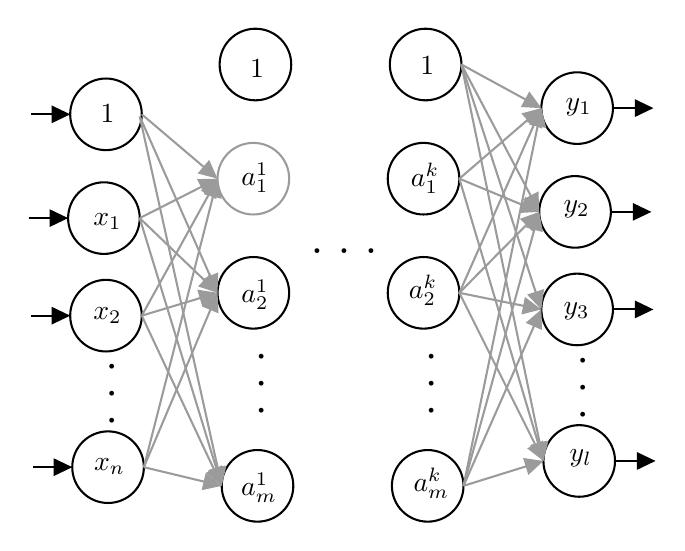
\begin{tikzpicture}[x=0.75pt,y=0.75pt,yscale=-1,xscale=1]
%uncomment if require: \path (0,300); %set diagram left start at 0, and has height of 300

%Shape: Circle [id:dp5524582775574844] 
\draw   (88,72.25) .. controls (88,62.72) and (95.72,55) .. (105.25,55) .. controls (114.78,55) and (122.5,62.72) .. (122.5,72.25) .. controls (122.5,81.78) and (114.78,89.5) .. (105.25,89.5) .. controls (95.72,89.5) and (88,81.78) .. (88,72.25) -- cycle ;
%Shape: Circle [id:dp9055284592778006] 
\draw   (89,242.25) .. controls (89,232.72) and (96.72,225) .. (106.25,225) .. controls (115.78,225) and (123.5,232.72) .. (123.5,242.25) .. controls (123.5,251.78) and (115.78,259.5) .. (106.25,259.5) .. controls (96.72,259.5) and (89,251.78) .. (89,242.25) -- cycle ;
%Shape: Circle [id:dp1656948629963515] 
\draw   (87,122.25) .. controls (87,112.72) and (94.72,105) .. (104.25,105) .. controls (113.78,105) and (121.5,112.72) .. (121.5,122.25) .. controls (121.5,131.78) and (113.78,139.5) .. (104.25,139.5) .. controls (94.72,139.5) and (87,131.78) .. (87,122.25) -- cycle ;
%Shape: Circle [id:dp606031338973398] 
\draw   (88,169.25) .. controls (88,159.72) and (95.72,152) .. (105.25,152) .. controls (114.78,152) and (122.5,159.72) .. (122.5,169.25) .. controls (122.5,178.78) and (114.78,186.5) .. (105.25,186.5) .. controls (95.72,186.5) and (88,178.78) .. (88,169.25) -- cycle ;
%Straight Lines [id:da7583336175527668] 
\draw    (69.02,72.25) -- (86,72.25) ;
\draw [shift={(88,72.25)}, rotate = 180] [fill={rgb, 255:red, 0; green, 0; blue, 0 }  ][line width=0.75]  [draw opacity=0] (8.93,-4.29) -- (0,0) -- (8.93,4.29) -- cycle    ;

%Straight Lines [id:da33136749911196883] 
\draw    (68.02,122.25) -- (85,122.25) ;
\draw [shift={(87,122.25)}, rotate = 180] [fill={rgb, 255:red, 0; green, 0; blue, 0 }  ][line width=0.75]  [draw opacity=0] (8.93,-4.29) -- (0,0) -- (8.93,4.29) -- cycle    ;

%Straight Lines [id:da4263129214891306] 
\draw    (69.02,169.25) -- (86,169.25) ;
\draw [shift={(88,169.25)}, rotate = 180] [fill={rgb, 255:red, 0; green, 0; blue, 0 }  ][line width=0.75]  [draw opacity=0] (8.93,-4.29) -- (0,0) -- (8.93,4.29) -- cycle    ;

%Straight Lines [id:da05901696855647298] 
\draw    (70.02,242.25) -- (87,242.25) ;
\draw [shift={(89,242.25)}, rotate = 180] [fill={rgb, 255:red, 0; green, 0; blue, 0 }  ][line width=0.75]  [draw opacity=0] (8.93,-4.29) -- (0,0) -- (8.93,4.29) -- cycle    ;

%Shape: Circle [id:dp7811394509655811] 
\draw   (160,48.25) .. controls (160,38.72) and (167.72,31) .. (177.25,31) .. controls (186.78,31) and (194.5,38.72) .. (194.5,48.25) .. controls (194.5,57.78) and (186.78,65.5) .. (177.25,65.5) .. controls (167.72,65.5) and (160,57.78) .. (160,48.25) -- cycle ;
%Shape: Circle [id:dp9905693780000109] 
\draw   (161,251.25) .. controls (161,241.72) and (168.72,234) .. (178.25,234) .. controls (187.78,234) and (195.5,241.72) .. (195.5,251.25) .. controls (195.5,260.78) and (187.78,268.5) .. (178.25,268.5) .. controls (168.72,268.5) and (161,260.78) .. (161,251.25) -- cycle ;
%Shape: Circle [id:dp10282768320714131] 
\draw  [color={rgb, 255:red, 155; green, 155; blue, 155 }  ,draw opacity=1 ] (159,103.25) .. controls (159,93.72) and (166.72,86) .. (176.25,86) .. controls (185.78,86) and (193.5,93.72) .. (193.5,103.25) .. controls (193.5,112.78) and (185.78,120.5) .. (176.25,120.5) .. controls (166.72,120.5) and (159,112.78) .. (159,103.25) -- cycle ;
%Shape: Circle [id:dp8751704729152276] 
\draw   (159,158.25) .. controls (159,148.72) and (166.72,141) .. (176.25,141) .. controls (185.78,141) and (193.5,148.72) .. (193.5,158.25) .. controls (193.5,167.78) and (185.78,175.5) .. (176.25,175.5) .. controls (166.72,175.5) and (159,167.78) .. (159,158.25) -- cycle ;
%Shape: Circle [id:dp14191125242712754] 
\draw   (242,48.25) .. controls (242,38.72) and (249.72,31) .. (259.25,31) .. controls (268.78,31) and (276.5,38.72) .. (276.5,48.25) .. controls (276.5,57.78) and (268.78,65.5) .. (259.25,65.5) .. controls (249.72,65.5) and (242,57.78) .. (242,48.25) -- cycle ;
%Shape: Circle [id:dp5157180132102686] 
\draw   (243,251.25) .. controls (243,241.72) and (250.72,234) .. (260.25,234) .. controls (269.78,234) and (277.5,241.72) .. (277.5,251.25) .. controls (277.5,260.78) and (269.78,268.5) .. (260.25,268.5) .. controls (250.72,268.5) and (243,260.78) .. (243,251.25) -- cycle ;
%Shape: Circle [id:dp8690128913833901] 
\draw   (241,103.25) .. controls (241,93.72) and (248.72,86) .. (258.25,86) .. controls (267.78,86) and (275.5,93.72) .. (275.5,103.25) .. controls (275.5,112.78) and (267.78,120.5) .. (258.25,120.5) .. controls (248.72,120.5) and (241,112.78) .. (241,103.25) -- cycle ;
%Shape: Circle [id:dp9649278733196962] 
\draw   (241,158.25) .. controls (241,148.72) and (248.72,141) .. (258.25,141) .. controls (267.78,141) and (275.5,148.72) .. (275.5,158.25) .. controls (275.5,167.78) and (267.78,175.5) .. (258.25,175.5) .. controls (248.72,175.5) and (241,167.78) .. (241,158.25) -- cycle ;
%Shape: Circle [id:dp1953350433383112] 
\draw   (315,69.25) .. controls (315,59.72) and (322.72,52) .. (332.25,52) .. controls (341.78,52) and (349.5,59.72) .. (349.5,69.25) .. controls (349.5,78.78) and (341.78,86.5) .. (332.25,86.5) .. controls (322.72,86.5) and (315,78.78) .. (315,69.25) -- cycle ;
%Shape: Circle [id:dp31843323470147866] 
\draw   (316,239.25) .. controls (316,229.72) and (323.72,222) .. (333.25,222) .. controls (342.78,222) and (350.5,229.72) .. (350.5,239.25) .. controls (350.5,248.78) and (342.78,256.5) .. (333.25,256.5) .. controls (323.72,256.5) and (316,248.78) .. (316,239.25) -- cycle ;
%Shape: Circle [id:dp7000306624407344] 
\draw   (314,119.25) .. controls (314,109.72) and (321.72,102) .. (331.25,102) .. controls (340.78,102) and (348.5,109.72) .. (348.5,119.25) .. controls (348.5,128.78) and (340.78,136.5) .. (331.25,136.5) .. controls (321.72,136.5) and (314,128.78) .. (314,119.25) -- cycle ;
%Shape: Circle [id:dp10864162142112854] 
\draw   (315,166.25) .. controls (315,156.72) and (322.72,149) .. (332.25,149) .. controls (341.78,149) and (349.5,156.72) .. (349.5,166.25) .. controls (349.5,175.78) and (341.78,183.5) .. (332.25,183.5) .. controls (322.72,183.5) and (315,175.78) .. (315,166.25) -- cycle ;
%Straight Lines [id:da9597423511061334] 
\draw    (350.02,69.25) -- (367,69.25) ;
\draw [shift={(369,69.25)}, rotate = 180] [fill={rgb, 255:red, 0; green, 0; blue, 0 }  ][line width=0.75]  [draw opacity=0] (8.93,-4.29) -- (0,0) -- (8.93,4.29) -- cycle    ;

%Straight Lines [id:da05206380931890586] 
\draw    (349.02,119.25) -- (366,119.25) ;
\draw [shift={(368,119.25)}, rotate = 180] [fill={rgb, 255:red, 0; green, 0; blue, 0 }  ][line width=0.75]  [draw opacity=0] (8.93,-4.29) -- (0,0) -- (8.93,4.29) -- cycle    ;

%Straight Lines [id:da5095484827545105] 
\draw    (350.02,166.25) -- (367,166.25) ;
\draw [shift={(369,166.25)}, rotate = 180] [fill={rgb, 255:red, 0; green, 0; blue, 0 }  ][line width=0.75]  [draw opacity=0] (8.93,-4.29) -- (0,0) -- (8.93,4.29) -- cycle    ;

%Straight Lines [id:da6172822793664112] 
\draw    (351.02,239.25) -- (368,239.25) ;
\draw [shift={(370,239.25)}, rotate = 180] [fill={rgb, 255:red, 0; green, 0; blue, 0 }  ][line width=0.75]  [draw opacity=0] (8.93,-4.29) -- (0,0) -- (8.93,4.29) -- cycle    ;

%Straight Lines [id:da8294435479357769] 
\draw [color={rgb, 255:red, 155; green, 155; blue, 155 }  ,draw opacity=1 ]   (122.5,72.25) -- (157.48,101.96) ;
\draw [shift={(159,103.25)}, rotate = 220.34] [fill={rgb, 255:red, 155; green, 155; blue, 155 }  ,fill opacity=1 ][line width=0.75]  [draw opacity=0] (8.93,-4.29) -- (0,0) -- (8.93,4.29) -- cycle    ;

%Straight Lines [id:da6143981027876961] 
\draw [color={rgb, 255:red, 155; green, 155; blue, 155 }  ,draw opacity=1 ]   (121.5,122.25) -- (157.22,104.15) ;
\draw [shift={(159,103.25)}, rotate = 513.13] [fill={rgb, 255:red, 155; green, 155; blue, 155 }  ,fill opacity=1 ][line width=0.75]  [draw opacity=0] (8.93,-4.29) -- (0,0) -- (8.93,4.29) -- cycle    ;

%Straight Lines [id:da8989735465663513] 
\draw [color={rgb, 255:red, 155; green, 155; blue, 155 }  ,draw opacity=1 ]   (122.5,169.25) -- (158.03,105) ;
\draw [shift={(159,103.25)}, rotate = 478.94] [fill={rgb, 255:red, 155; green, 155; blue, 155 }  ,fill opacity=1 ][line width=0.75]  [draw opacity=0] (8.93,-4.29) -- (0,0) -- (8.93,4.29) -- cycle    ;

%Straight Lines [id:da18190387914988415] 
\draw [color={rgb, 255:red, 155; green, 155; blue, 155 }  ,draw opacity=1 ]   (123.5,242.25) -- (158.51,105.19) ;
\draw [shift={(159,103.25)}, rotate = 464.33] [fill={rgb, 255:red, 155; green, 155; blue, 155 }  ,fill opacity=1 ][line width=0.75]  [draw opacity=0] (8.93,-4.29) -- (0,0) -- (8.93,4.29) -- cycle    ;

%Straight Lines [id:da982035899456049] 
\draw [color={rgb, 255:red, 155; green, 155; blue, 155 }  ,draw opacity=1 ]   (121.5,73.25) -- (158.19,156.42) ;
\draw [shift={(159,158.25)}, rotate = 246.19] [fill={rgb, 255:red, 155; green, 155; blue, 155 }  ,fill opacity=1 ][line width=0.75]  [draw opacity=0] (8.93,-4.29) -- (0,0) -- (8.93,4.29) -- cycle    ;

%Straight Lines [id:da71035902210412] 
\draw [color={rgb, 255:red, 155; green, 155; blue, 155 }  ,draw opacity=1 ]   (121.5,73.25) -- (160.57,249.3) ;
\draw [shift={(161,251.25)}, rotate = 257.49] [fill={rgb, 255:red, 155; green, 155; blue, 155 }  ,fill opacity=1 ][line width=0.75]  [draw opacity=0] (8.93,-4.29) -- (0,0) -- (8.93,4.29) -- cycle    ;

%Straight Lines [id:da8313033107784724] 
\draw [color={rgb, 255:red, 155; green, 155; blue, 155 }  ,draw opacity=1 ]   (121.5,122.25) -- (157.56,156.86) ;
\draw [shift={(159,158.25)}, rotate = 223.82999999999998] [fill={rgb, 255:red, 155; green, 155; blue, 155 }  ,fill opacity=1 ][line width=0.75]  [draw opacity=0] (8.93,-4.29) -- (0,0) -- (8.93,4.29) -- cycle    ;

%Straight Lines [id:da9551803570009156] 
\draw [color={rgb, 255:red, 155; green, 155; blue, 155 }  ,draw opacity=1 ]   (121.5,122.25) -- (160.41,249.34) ;
\draw [shift={(161,251.25)}, rotate = 252.98000000000002] [fill={rgb, 255:red, 155; green, 155; blue, 155 }  ,fill opacity=1 ][line width=0.75]  [draw opacity=0] (8.93,-4.29) -- (0,0) -- (8.93,4.29) -- cycle    ;

%Straight Lines [id:da38817861817600297] 
\draw [color={rgb, 255:red, 155; green, 155; blue, 155 }  ,draw opacity=1 ]   (122.5,169.25) -- (157.09,158.83) ;
\draw [shift={(159,158.25)}, rotate = 523.23] [fill={rgb, 255:red, 155; green, 155; blue, 155 }  ,fill opacity=1 ][line width=0.75]  [draw opacity=0] (8.93,-4.29) -- (0,0) -- (8.93,4.29) -- cycle    ;

%Straight Lines [id:da8106157570982881] 
\draw [color={rgb, 255:red, 155; green, 155; blue, 155 }  ,draw opacity=1 ]   (122.5,169.25) -- (160.15,249.44) ;
\draw [shift={(161,251.25)}, rotate = 244.85] [fill={rgb, 255:red, 155; green, 155; blue, 155 }  ,fill opacity=1 ][line width=0.75]  [draw opacity=0] (8.93,-4.29) -- (0,0) -- (8.93,4.29) -- cycle    ;

%Straight Lines [id:da8506194325261827] 
\draw [color={rgb, 255:red, 155; green, 155; blue, 155 }  ,draw opacity=1 ]   (123.5,242.25) -- (158.22,160.09) ;
\draw [shift={(159,158.25)}, rotate = 472.91] [fill={rgb, 255:red, 155; green, 155; blue, 155 }  ,fill opacity=1 ][line width=0.75]  [draw opacity=0] (8.93,-4.29) -- (0,0) -- (8.93,4.29) -- cycle    ;

%Straight Lines [id:da20779122573633657] 
\draw [color={rgb, 255:red, 155; green, 155; blue, 155 }  ,draw opacity=1 ]   (123.5,242.25) -- (159.06,250.78) ;
\draw [shift={(161,251.25)}, rotate = 193.5] [fill={rgb, 255:red, 155; green, 155; blue, 155 }  ,fill opacity=1 ][line width=0.75]  [draw opacity=0] (8.93,-4.29) -- (0,0) -- (8.93,4.29) -- cycle    ;

%Straight Lines [id:da04429768381781707] 
\draw [color={rgb, 255:red, 155; green, 155; blue, 155 }  ,draw opacity=1 ]   (276.5,48.25) -- (313.24,68.29) ;
\draw [shift={(315,69.25)}, rotate = 208.61] [fill={rgb, 255:red, 155; green, 155; blue, 155 }  ,fill opacity=1 ][line width=0.75]  [draw opacity=0] (8.93,-4.29) -- (0,0) -- (8.93,4.29) -- cycle    ;

%Straight Lines [id:da5973417342423057] 
\draw [color={rgb, 255:red, 155; green, 155; blue, 155 }  ,draw opacity=1 ]   (276.5,48.25) -- (313.07,117.48) ;
\draw [shift={(314,119.25)}, rotate = 242.16] [fill={rgb, 255:red, 155; green, 155; blue, 155 }  ,fill opacity=1 ][line width=0.75]  [draw opacity=0] (8.93,-4.29) -- (0,0) -- (8.93,4.29) -- cycle    ;

%Straight Lines [id:da6660645274660697] 
\draw [color={rgb, 255:red, 155; green, 155; blue, 155 }  ,draw opacity=1 ]   (276.5,48.25) -- (314.38,164.35) ;
\draw [shift={(315,166.25)}, rotate = 251.93] [fill={rgb, 255:red, 155; green, 155; blue, 155 }  ,fill opacity=1 ][line width=0.75]  [draw opacity=0] (8.93,-4.29) -- (0,0) -- (8.93,4.29) -- cycle    ;

%Straight Lines [id:da15404201533057482] 
\draw [color={rgb, 255:red, 155; green, 155; blue, 155 }  ,draw opacity=1 ]   (276.5,48.25) -- (315.59,237.29) ;
\draw [shift={(316,239.25)}, rotate = 258.32] [fill={rgb, 255:red, 155; green, 155; blue, 155 }  ,fill opacity=1 ][line width=0.75]  [draw opacity=0] (8.93,-4.29) -- (0,0) -- (8.93,4.29) -- cycle    ;

%Straight Lines [id:da42172561870037417] 
\draw [color={rgb, 255:red, 155; green, 155; blue, 155 }  ,draw opacity=1 ]   (275.5,103.25) -- (313.48,70.55) ;
\draw [shift={(315,69.25)}, rotate = 499.28] [fill={rgb, 255:red, 155; green, 155; blue, 155 }  ,fill opacity=1 ][line width=0.75]  [draw opacity=0] (8.93,-4.29) -- (0,0) -- (8.93,4.29) -- cycle    ;

%Straight Lines [id:da45826700040495716] 
\draw [color={rgb, 255:red, 155; green, 155; blue, 155 }  ,draw opacity=1 ]   (275.5,103.25) -- (312.15,118.48) ;
\draw [shift={(314,119.25)}, rotate = 202.57] [fill={rgb, 255:red, 155; green, 155; blue, 155 }  ,fill opacity=1 ][line width=0.75]  [draw opacity=0] (8.93,-4.29) -- (0,0) -- (8.93,4.29) -- cycle    ;

%Straight Lines [id:da7789429248333253] 
\draw [color={rgb, 255:red, 155; green, 155; blue, 155 }  ,draw opacity=1 ]   (275.5,103.25) -- (315.43,237.33) ;
\draw [shift={(316,239.25)}, rotate = 253.42000000000002] [fill={rgb, 255:red, 155; green, 155; blue, 155 }  ,fill opacity=1 ][line width=0.75]  [draw opacity=0] (8.93,-4.29) -- (0,0) -- (8.93,4.29) -- cycle    ;

%Straight Lines [id:da8873311658686183] 
\draw [color={rgb, 255:red, 155; green, 155; blue, 155 }  ,draw opacity=1 ]   (275.5,158.25) -- (314.19,71.08) ;
\draw [shift={(315,69.25)}, rotate = 473.93] [fill={rgb, 255:red, 155; green, 155; blue, 155 }  ,fill opacity=1 ][line width=0.75]  [draw opacity=0] (8.93,-4.29) -- (0,0) -- (8.93,4.29) -- cycle    ;

%Straight Lines [id:da17581141425949265] 
\draw [color={rgb, 255:red, 155; green, 155; blue, 155 }  ,draw opacity=1 ]   (275.5,158.25) -- (312.59,120.67) ;
\draw [shift={(314,119.25)}, rotate = 494.63] [fill={rgb, 255:red, 155; green, 155; blue, 155 }  ,fill opacity=1 ][line width=0.75]  [draw opacity=0] (8.93,-4.29) -- (0,0) -- (8.93,4.29) -- cycle    ;

%Straight Lines [id:da9574684180353887] 
\draw [color={rgb, 255:red, 155; green, 155; blue, 155 }  ,draw opacity=1 ]   (275.5,158.25) -- (313.04,165.85) ;
\draw [shift={(315,166.25)}, rotate = 191.45] [fill={rgb, 255:red, 155; green, 155; blue, 155 }  ,fill opacity=1 ][line width=0.75]  [draw opacity=0] (8.93,-4.29) -- (0,0) -- (8.93,4.29) -- cycle    ;

%Straight Lines [id:da07582757410341223] 
\draw [color={rgb, 255:red, 155; green, 155; blue, 155 }  ,draw opacity=1 ]   (275.5,158.25) -- (315.11,237.46) ;
\draw [shift={(316,239.25)}, rotate = 243.43] [fill={rgb, 255:red, 155; green, 155; blue, 155 }  ,fill opacity=1 ][line width=0.75]  [draw opacity=0] (8.93,-4.29) -- (0,0) -- (8.93,4.29) -- cycle    ;

%Straight Lines [id:da6744789233764286] 
\draw [color={rgb, 255:red, 155; green, 155; blue, 155 }  ,draw opacity=1 ]   (277.5,251.25) -- (314.6,71.21) ;
\draw [shift={(315,69.25)}, rotate = 461.64] [fill={rgb, 255:red, 155; green, 155; blue, 155 }  ,fill opacity=1 ][line width=0.75]  [draw opacity=0] (8.93,-4.29) -- (0,0) -- (8.93,4.29) -- cycle    ;

%Straight Lines [id:da25721287639161394] 
\draw [color={rgb, 255:red, 155; green, 155; blue, 155 }  ,draw opacity=1 ]   (277.5,251.25) -- (313.47,121.18) ;
\draw [shift={(314,119.25)}, rotate = 465.46] [fill={rgb, 255:red, 155; green, 155; blue, 155 }  ,fill opacity=1 ][line width=0.75]  [draw opacity=0] (8.93,-4.29) -- (0,0) -- (8.93,4.29) -- cycle    ;

%Straight Lines [id:da5800245371904054] 
\draw [color={rgb, 255:red, 155; green, 155; blue, 155 }  ,draw opacity=1 ]   (277.5,251.25) -- (314.19,168.08) ;
\draw [shift={(315,166.25)}, rotate = 473.81] [fill={rgb, 255:red, 155; green, 155; blue, 155 }  ,fill opacity=1 ][line width=0.75]  [draw opacity=0] (8.93,-4.29) -- (0,0) -- (8.93,4.29) -- cycle    ;

%Straight Lines [id:da7868222132265981] 
\draw [color={rgb, 255:red, 155; green, 155; blue, 155 }  ,draw opacity=1 ]   (277.5,251.25) -- (314.09,239.85) ;
\draw [shift={(316,239.25)}, rotate = 522.69] [fill={rgb, 255:red, 155; green, 155; blue, 155 }  ,fill opacity=1 ][line width=0.75]  [draw opacity=0] (8.93,-4.29) -- (0,0) -- (8.93,4.29) -- cycle    ;



% Text Node
\draw (108,207) node [rotate=-90] [align=left] {\textbf{{\large . . .}}};
% Text Node
\draw (180,202) node [rotate=-90] [align=left] {\textbf{{\large . . .}}};
% Text Node
\draw (220,138) node  [align=left] {\textbf{{\large . . .}}};
% Text Node
\draw (262,202) node [rotate=-90] [align=left] {\textbf{{\large . . .}}};
% Text Node
\draw (335,204) node [rotate=-90] [align=left] {\textbf{{\large . . .}}};
% Text Node
\draw (106,72) node   {$1$};
% Text Node
\draw (106,124) node   {$x_{1}$};
% Text Node
\draw (106,169) node   {$x_{2}$};
% Text Node
\draw (107,242) node   {$x_{n}$};
% Text Node
\draw (178,50) node   {$1$};
% Text Node
\draw (177,103) node   {$a^{1}_{1}$};
% Text Node
\draw (177,159) node   {$a^{1}_{2}$};
% Text Node
\draw (179,252) node   {$a^{1}_{m}$};
% Text Node
\draw (260,49) node   {$1$};
% Text Node
\draw (259,103) node   {$a^{k}_{1}$};
% Text Node
\draw (258,157) node   {$a^{k}_{2}$};
% Text Node
\draw (262,250) node   {$a^{k}_{m}$};
% Text Node
\draw (333,69) node   {$y_{1}$};
% Text Node
\draw (332,118) node   {$y_{2}$};
% Text Node
\draw (332,167) node   {$y_{3}$};
% Text Node
\draw (334,238) node   {$y_{l}$};


\end{tikzpicture}

	\caption{Arquitectura de la red neuronal \gls{mlp}.}
	\label{fig:redneuronal}
\end{figure}

\par Si se quiere expresar el funcionamiento de una red neuronal de forma matricial se puede hacer lo siguiente, si se observa la arquitectura de la red neuronal de la figura \ref{fig:redneuronal} se puede ver que las entradas $X$ pueden expresar de forma vectorial igual que las salidas $Y$ y los pesos $\theta$ también se puede expresar de forma matricial.
\begin{spreadlines}{10pt}
	\begin{alignat}{4}
		\label{eq:1}
		 & X=\begin{bmatrix}
			1     \\
			x_{1} \\
			x_{2} \\
			...   \\
			x_{n}
		\end{bmatrix}                \\  \label{eq:2}
		 & \Theta ^{1}_{j} =\begin{bmatrix}
			\theta ^{1}_{0j} \\
			\theta ^{1}_{1j} \\
			\theta ^{1}_{2j} \\
			.+..             \\
			\theta ^{1}_{nj}
		\end{bmatrix} \\ \label{eq:3}
		 & \Theta ^{i}_{j} =\begin{bmatrix}
			\theta ^{i}_{0j} \\
			\theta ^{i}_{1j} \\
			\theta ^{i}_{2j} \\
			...              \\
			\theta ^{i}_{mj}
		\end{bmatrix} \\ \label{eq:4}
		 & A^{i} =\begin{bmatrix}
			1         \\
			a^{i}_{1} \\
			a^{i}_{2} \\
			...       \\
			a^{i}_{m}
		\end{bmatrix}           \\
		 & \Theta ^{i} =\begin{bmatrix}
			\Theta ^{i}_{1} & \Theta ^{i}_{2} & ... & \Theta ^{i}_{m}\end{bmatrix}
	\end{alignat}
\end{spreadlines}

\par El superíndice indica la capa a la que pertenece, en el caso de los subíndices de $\Theta$ el primer dígito simboliza la neurona de la que procede y el siguiente es a la que entra. A partir de estas ecuaciones se puede ver que para obtener la matriz $A$ de la primera capa se debe usar esta ecuación:

\begin{equation*}
	A^{1} =F\left(\left( \Theta ^{1}\right)^{T} X\right)
\end{equation*}

\par Para obtener las matrices $A$ de cada capa se usa la siguiente ecuación:

\begin{equation*}
	A^{i} =F\left(\left( \Theta ^{i}\right)^{T} A^{i-1}\right)
\end{equation*}

\par En estas dos ecuaciones la función $F$ es la función no lineal que se deseé usar para la salida de cada neurona. En algunas de las aplicaciones se usan funciones como \gls{ReLU} la cual tiene una respuesta como la función escalón, en otras aplicación se usa la función sigmoidal, en otras ocasiones se usa el tangente hiperbólico, en la figura \ref{fig:funciones} se muestran algunas de las funciones más comunes que se usan en las aplicaciones.
\begin{figure}[h]
	\centering
	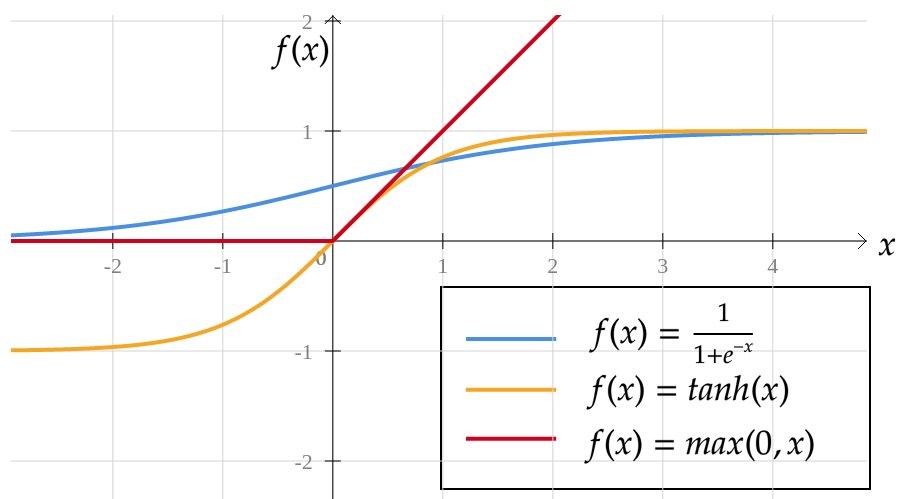
\includegraphics[width=0.7\textwidth]{imagenes/graficaF.png}
	\caption{Ejemplo de algunas de las salidas de una neurona artificial.}
	\label{fig:funciones}
\end{figure}
\par Por último la salida vectorial de la red neuronal se calcula usando la siguiente ecuación:

\begin{equation*}
	Y\ =F\left(\left( \Theta ^{k+1}\right)^{T} A^{k}\right)
\end{equation*}

\par Al proceso que obtiene la predicción en una red neuronal se le llama \textit{feedforward}.

\subsection{Fase de entrenamiento - optimación}

\par La fase entrenamiento de la red neuronal consiste en modificar los pesos $\theta$ que corresponden a cada neurona, esto se hace mediante un proceso llamado \gls{backpropagation}, éste consiste en modificar los pesos de la red de modo que se minimice la función de costo, por medio de la retroalimentación de la red hasta la primera capa. Esta idea fue por primera vez concebida por \textcite{rumelhart1986learning} en su artículo \textit{Learning representations by back-propagating errors}, en el cuál se calcula el error total que se veía a la salida de la red neuronal, y se obtiene con la ecuación \ref{eq:error}.

\begin{equation}\label{eq:error}
	E=\frac{1}{2}\sum _{c}\sum _{j}( y_{j,c} -d_{j,c})^{2}
\end{equation}

donde $c$ es índice sobre las muestras, $j$ es el índice sobre las unidades de salida, $y$ es el valor de salida de la red y $d$ es el valor deseado. Luego entonces si se minimiza este error el desempeño de la red neuronal con respecto al problema será mejor, este error es únicamente para la última capa, para esto es necesario derivar parcialmente la función del error con respecto a los pesos de las sinapsis de entrada de cada una de las unidades, para esto se puede ver el desarrollo que hizo \textcite{rumelhart1986learning} con respecto a la función sigmoidal.

\par Se deriva primero el error $E$ con respecto a $y_{j}$ en cada muestra $c$, por lo tanto se omite.
\begin{equation*}
	\frac{\partial E}{\partial y_{j}} =y_{j} -d_{j}
\end{equation*}
\par Esta parcial es únicamente para la última capa, después se verá como calcular el de las siguientes. Después se ve que con la regla de la cadena se puede tener lo siguiente:
\begin{equation*}
	\frac{\partial E}{\partial x_{j}} =\frac{\partial E}{\partial y_{j}}  \frac{\partial y_{j}}{\partial x_{j}}
\end{equation*}

En donde $y_{j}$ está dado por la función sigmoidal en este caso por lo tanto se sustituye la derivada parcial con respecto a $x_{j}$.
\begin{spreadlines}{10pt}
	\begin{alignat*}{4}
		 & y_{j} =\frac{1}{1+e^{-x_{j}}}                                                         \\
		 & \frac{\partial y_{j}}{\partial x_{j}} =\frac{e^{-x_{j}}}{1+e^{-x_{j}}}                \\
		 & \frac{\partial y_{j}}{\partial x_{j}}=y_{j} (1-y_{j})                                 \\
		 & \frac{\partial E}{\partial x_{j}} =\frac{\partial E}{\partial y_{j}}  y_{j}( 1-y_{j})
	\end{alignat*}
\end{spreadlines}

\par En esta parte se puede reemplazar la parcial cuando se usa la función \gls{ReLU} o la de la tangente hiperbólica. Después se puede hacer de nuevo la regla de la cadena para obtener la derivada parcial de error con respecto a los pesos.

\begin{spreadlines}{10pt}
	\begin{alignat*}{3}
		 & x_{j}=\sum_{i} y_{i}\theta_{ji}                                                                                          \\ \vspace{100pt}
		 & \frac{\partial E}{\partial \theta _{ji}} =\frac{\partial E}{\partial x_{j}} \frac{\partial x_{j}}{\partial \theta _{ji}} \\
		 & \frac{\partial E}{\partial \theta _{ji}} =\frac{\partial E}{\partial x_{j}}y_{i}
	\end{alignat*}
\end{spreadlines}

\par Después para conseguir la parcial del error con respecto a $x_{j}$ se debe hacer lo siguiente:

\begin{spreadlines}{10pt}
	\begin{alignat*}{3}
		 & \frac{\partial E}{\partial x_{j}} \frac{\partial x_{j}}{\partial y_{i}} =\frac{\partial E}{\partial x_{j}} \theta _{ji} \\
		 & \frac{\partial E}{\partial y_{j}} =\sum _{j}\frac{\partial E}{\partial x_{j}} \theta _{ji}
	\end{alignat*}
\end{spreadlines}

\par Con este resultado se puede calcular progresivamente las derivadas parciales del error con respecto a los pesos, en otras palabras la razón de cambio del error con respecto a la modificación de los pesos. Lo que indica hacia donde está el mínimo local. Entonces para encontrar el incremento de los pesos $\theta$ se puede aplicar la siguiente ecuación:
\[ \Delta \theta =-\epsilon \frac{\partial E}{\partial \theta }\]

\par En esta ecuación $\epsilon$ simboliza el coeficiente de aprendizaje el cual indica que tan rápido se avanzará hacia el mínimo local. Este valor también se puede poner en función del tiempo de modo que a medida que se acerque al valor se vuelve más pequeño el paso. Este método fue primeramente descrito por \textcite{rumelhart1986learning} y tiene una desventaja muy importante, para actualizar una vez los nuevos pesos es necesario computar el error de todas las muestras, por lo tanto tardará un tiempo considerable en terminar una actualización si se tienen muchas muestras, las cuales son necesarias en la mayoría de los casos para encontrar un buen modelo que generalice el problema.

\par Este algoritmo de optimación tendrá un gran precio computacional, para este propósito se creó el \gls{SGD} el cual para actualizar los pesos en la red neuronal se obtiene el gradiente de un conjunto aleatorio de muestras, y no es necesario computar el gradiente de todo el conjunto de datos. Sin embargo, este método tiene la desventaja que no se encuentra el gradiente general que describirían todas las muestras, sino una aproximación, por lo que el coeficiente de aprendizaje debe ser más pequeño y deberán hacerse más actualizaciones.

\par Otra opción que surgió con el tiempo fue dotar al cambio de los pesos de un momento esto para que aún cuando había encontrado un mínimo local, el paso pudiera pasarlo por alto con la intención de buscar uno que estuviera en la vecindad, este método no resultó tan bueno ya que podía estancarse en zonas llanas aún más altas que el mínimo local que había ignorado. Luego de este método surgió otro que consideraría una adaptación a las condiciones del gradiente, es decir que en zonas donde fuera necesario que $\epsilon$ fuera más pequeño para conseguir converger, pudiera adaptarse, entonces surgió Adagrad. Luego se pensó que se podría hacer variar de igual modo el momento ese fue el surgimiento de Adam, el cual es el método usado en esta tesis, no se pensó en probar con otros ya que Adam ha reportado mejores resultados en la literatura que sus alternativas, este método fue ideado por \textcite{kingma2014adam}.  Sin embargo, como se ha visto en diferentes investigaciones, los mejores resultados se obtienen al usar como optimizador el Root Mean Square(RMS) el cual es un Gradient Descent con momento.
\nocite{DBLP:journals/corr/Ruder16}


\subsection{Éxito del método}

\par Las redes neuronales han sido ocupadas para muchas aplicaciones hoy en día, sin embargo, en sus inicios en 1943 cuando \textcite{mcculloch1943logical} investigaba como guardaba información no se pensaba que sería tan utilizado, fue con \textcite{rosenblatt1958perceptron} 15 años después cuando apenas se vería un avance significativo con respecto a lo son qué hoy día, incluso se construyeron proyectos como Mark 1 perceptron. Sin embargo, los proyectos que llegaban a ver la luz, apenas podían distinguir entre clases y con un desempeño precario, debido principalmente al poder de cómputo que es necesario para entrenarlas, fue más bien a partir de los años 2000 con la entrada al mercado y el desarrollo de las API por parte de NVIDIA, AMD e INTEL que la investigación comenzó a tomar el impulso que necesitaba, ahora existen muchas API de desarrollo de sistemas inteligentes como Keras, Tensorflow, Sklearn, etc. con un continuo crecimiento. Hoy en día las redes neuronales son el algoritmo número uno bio-inspirado que los investigadores usan para hacer sus experimentos (63.04\% en el 2016). Como lo menciona \textcite{kar2016bio} existen muchos más algoritmos que se pueden explorar más como Artificial Plant Optimization, pero aún por mucho tiempo se prevé que las redes neuronales controlen el mercado y las investigaciones científicas gracias a que aportan resultados confiables y de rápido desarrollo sin la necesidad de conocer rigurosamente las matemáticas detrás de ellas.

\par Entre los usos que se les han dado están los siguientes: en el artículo \textit{Performance Analysis of Domestic Refrigerator Using Hydrocarbon Refrigerant Mixtures with ANN} de \textcite{reddy2019performance} lo usan para analizar el rendimiento de un refrigerador usando diferentes refrigerantes, en el artículo \textit{Assessing the culture of fruit farmers from Calvillo, Aguascalientes, Mexico with an artificial neural network: An approximation of sustainable land management} de \textcite{santos2019assessing} se buscan soluciones para el cultivo sustentable en la región de Calvillo en Aguascalientes, en el artículo \textit{LED color prediction using a boosting neural network model for a visual-MIMO system} de \textcite{banik2018led} se usa un modelo de red neuronal que predice el color de un LED, entre otras.

\subsection{Redes bidireccionales de gran memoria de corto plazo}

\par Como se vio en la sección anterior las redes neuronales han servido ampliamente a muchas áreas del conocimiento, sin embargo, para cada uno de los problemas se debe usar una arquitectura de red neuronal que sea apropiada y que justifique que puede resolver el problema. Esta arquitectura no siempre es fácil encontrarla y muchas veces es necesario probar con más de una arquitectura con el fin de comparar resultados y decidirse por una. En otros casos es necesario utilizar modelos de forma secuencial de manera que la salida de uno sea la entrada de otro, como se puede ver, no existe nada escrito en cuanto al diseño que debe tener un modelo para resolver determinado problema. A continuación se explicará un poco sobre la arquitectura que se uso en el problema y la justificación que se tuvo en mente.

\par Para explicar una \gls{bi-lstm} primero se debe abordar ¿Qué es una red neuronal recurrente?¿Qué es una LSTM?

\par Una red neuronal recurrente es una red neuronal cuyas neuronas tienen una entrada secuencial; por ejemplo, una serie de palabras, una serie de carácteres, de imágenes etc. Lo que se busca con esta arquitectura es que las neuronas tengan una forma de retener información sobre los datos que han sido vistos, por lo que se puede decir que posee la capacidad de tener memoria, el modelo de esa neurona es el que se muestra en la figura \ref{fig:3.10}:

\begin{figure}[H]
	\centering
	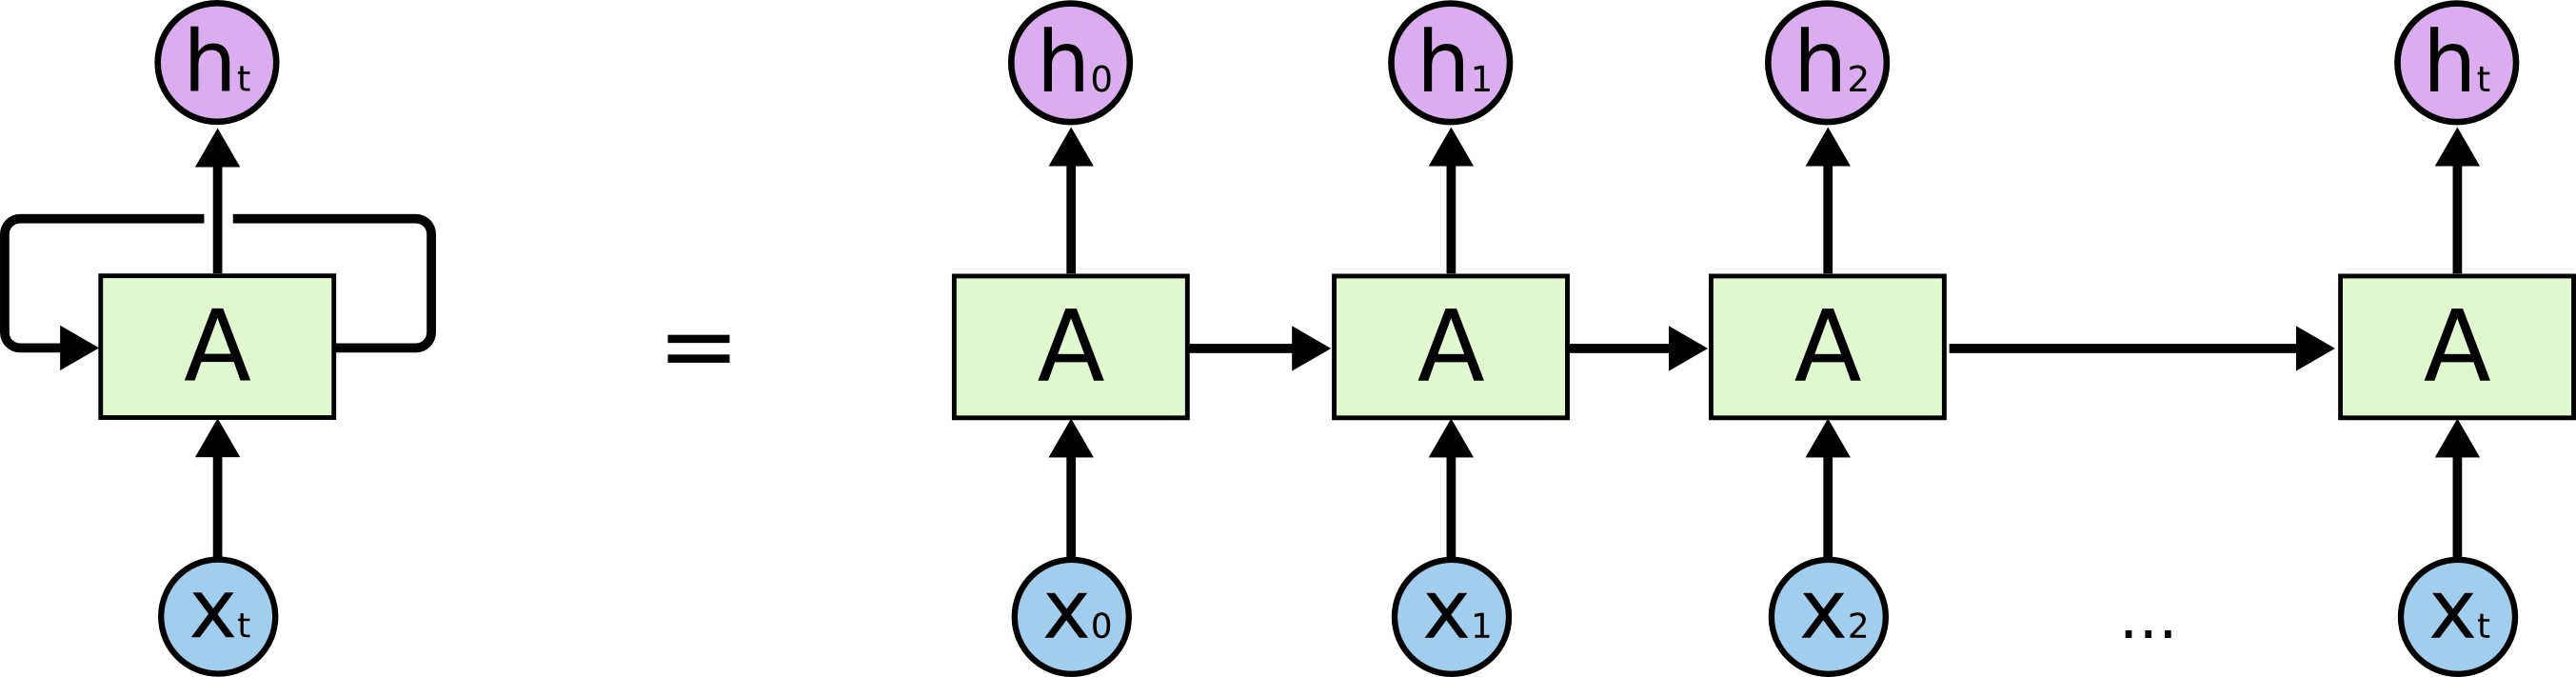
\includegraphics[width=\textwidth]{imagenes/RNN-unrolled.png}
	\caption[]{Modelo de una red neuronal recurrente. (Imagen extraída de \textcite{christopher_olah_2015}) }
	\label{fig:3.10}
\end{figure}

\par El problema principal de que las neuronas guarden toda la información de lo que han visto es que en muchos casos es mucho más relevante la información actual que todo lo que se ha visto anteriormente; por ejemplo, si en el conjunto de muestras se tiene un tweet que contiene lo siguiente:
\vspace{5pt}
\begin{center}
	\textit{``Ayer me desperté temprano para ir a trabajar y cuando llegué ahí me dí cuenta que era sábado, de regreso a mi casa se me recargo una señora en el metro, gracias reloj \#thanks''},
	\label{fig:frase}
\end{center}
\vspace{5pt}

\par En este texto se puede ver que si la red neuronal esta recordando todo lo que ve, entonces ésta ``considera'' que para identificar algo como sarcasmo es igual de relevante la parte en la que se le recargo una señora que haber ido a su empleo en su día de descanso. Para dicha tarea en la que la información puede o no ser relevante se tiene la \gls{lstm} las cuales tiene una estructura similar a la que se muestra en la figura \ref{fig:3.11}:

\begin{figure}[H]
	\centering
	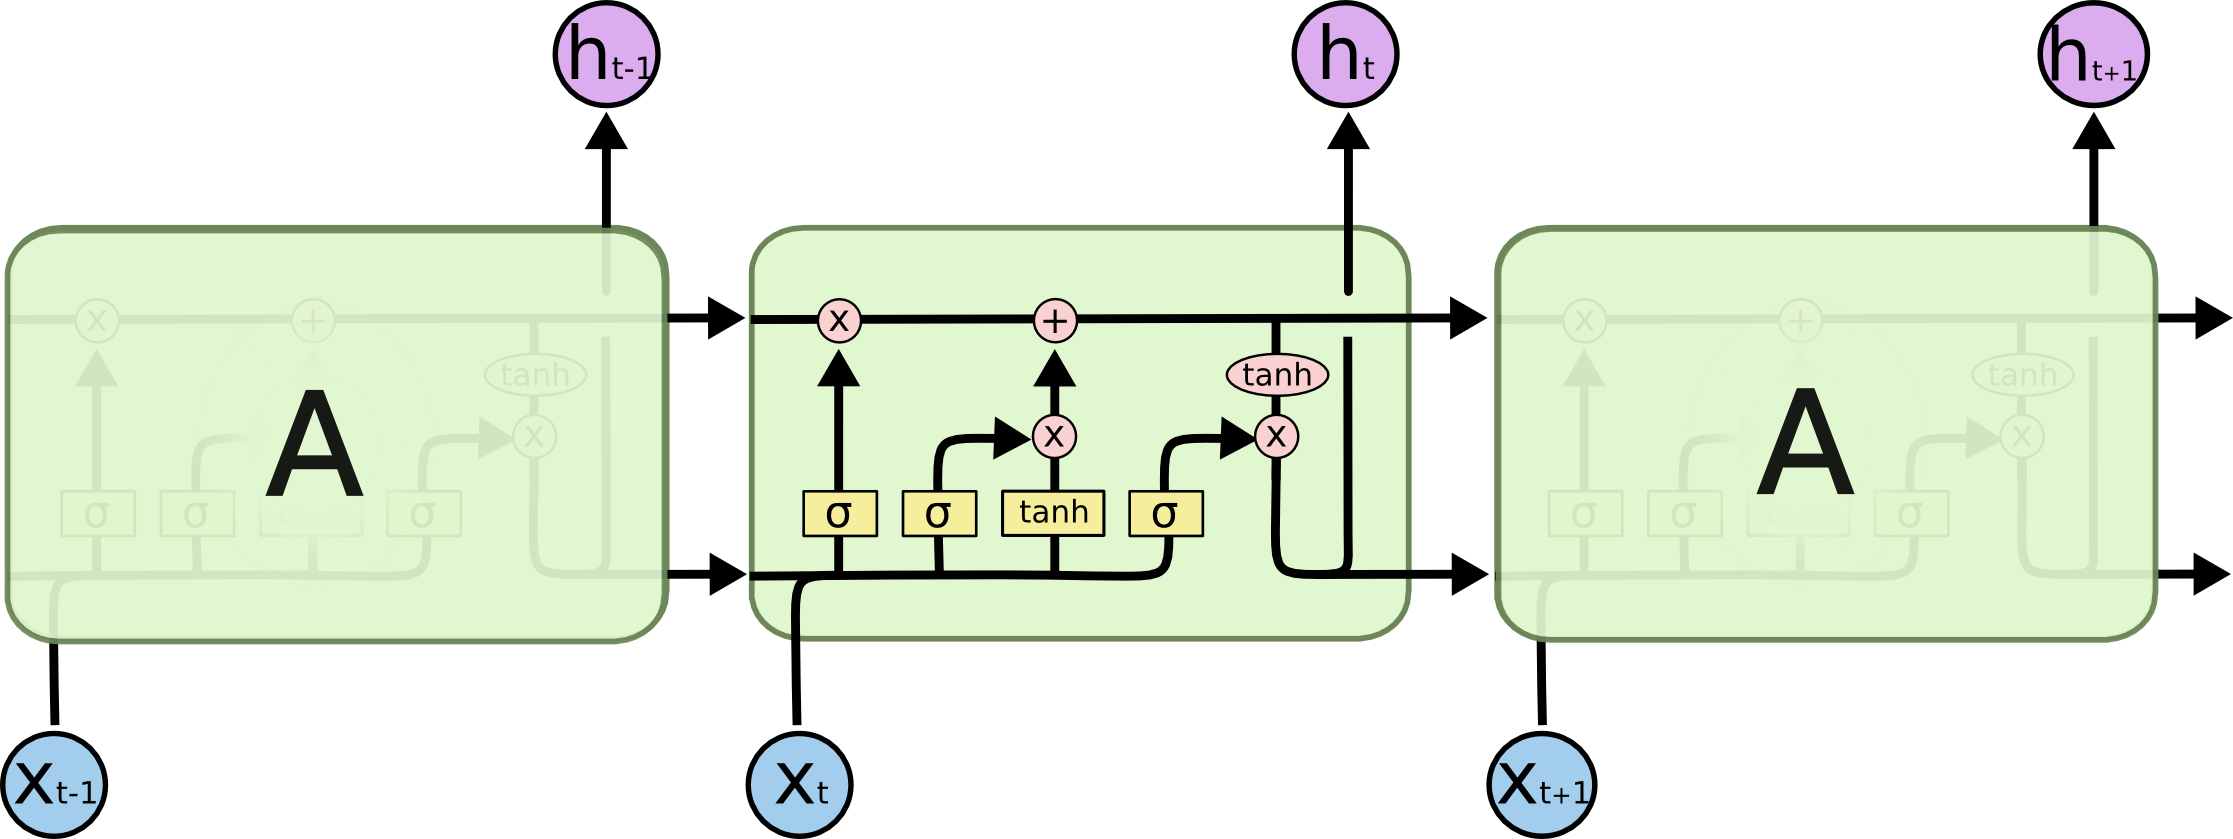
\includegraphics[width=\textwidth]{imagenes/LSTM3-chain.png}
	\caption[]{Arquitectura de una \gls{lstm}. (Imagen extraída de \textcite{christopher_olah_2015})}
	\label{fig:3.11}
\end{figure}


\par Esta arquitectura tiene diferentes partes, dentro de las cuales se pueden distinguir las siguientes: la parte que decide si olvidar o no, la parte que añade el concepto actual al concepto acumulado y la parte que pasa los parámetros de salida a la entrada de la siguiente unidad.

\begin{figure}[H]
	\centering
	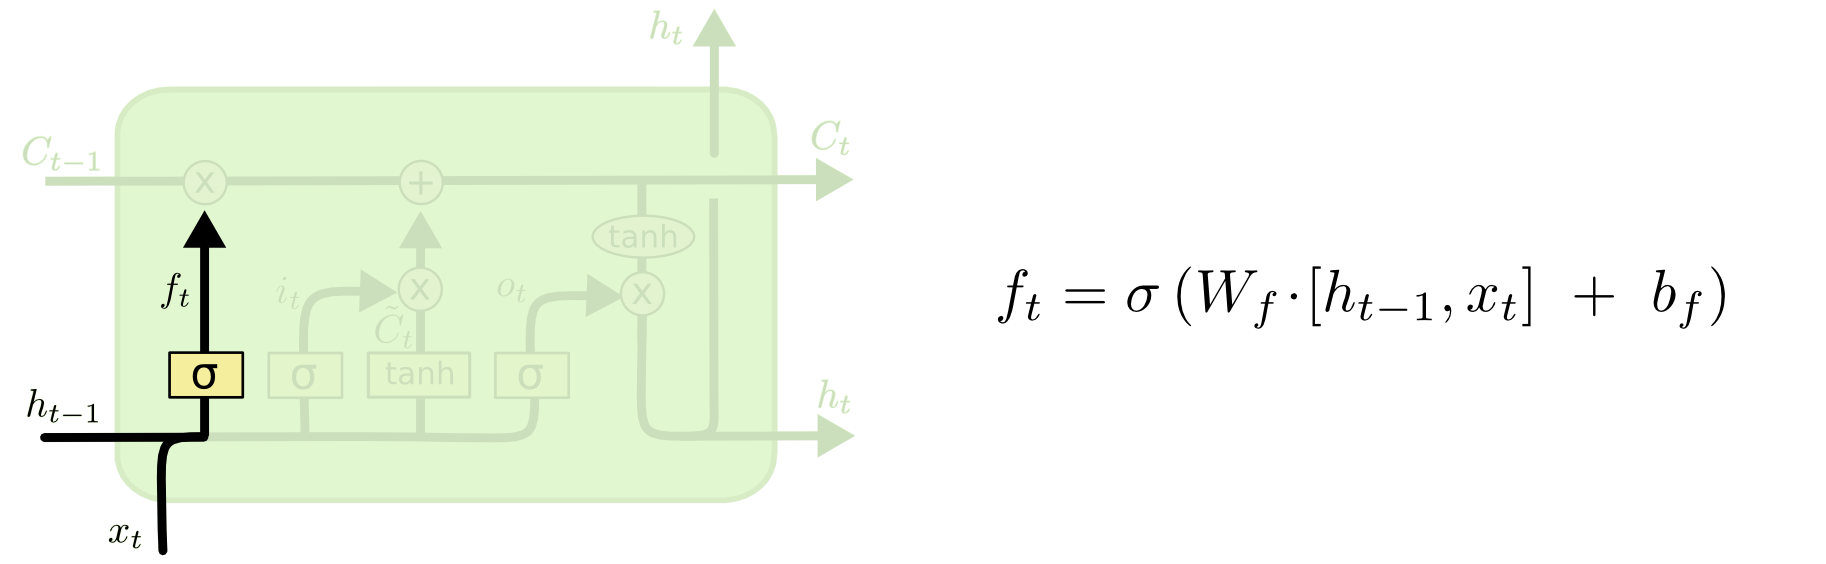
\includegraphics[width=\textwidth]{imagenes/LSTM3-focus-f.png}
	\caption[]{Sección de la unidad \gls{lstm} que decide si olvida o no.(Imagen extraída de \textcite{christopher_olah_2015})}
	\label{fig:lstmOlvidar}
\end{figure}


\par En la figura \ref{fig:lstmOlvidar} $\sigma$ es la función sigmoidal que recibe la concatenación del valor que le aporta la unidad anterior y la información que actualmente puede ver, y tiene el propósito de pasar a la unidad que multiplica un valor cercano a 1, que indica que recordará todo lo que ha visto, o un valor 0 para borrar completamente lo que había visto.

\begin{figure}[H]
	\centering
	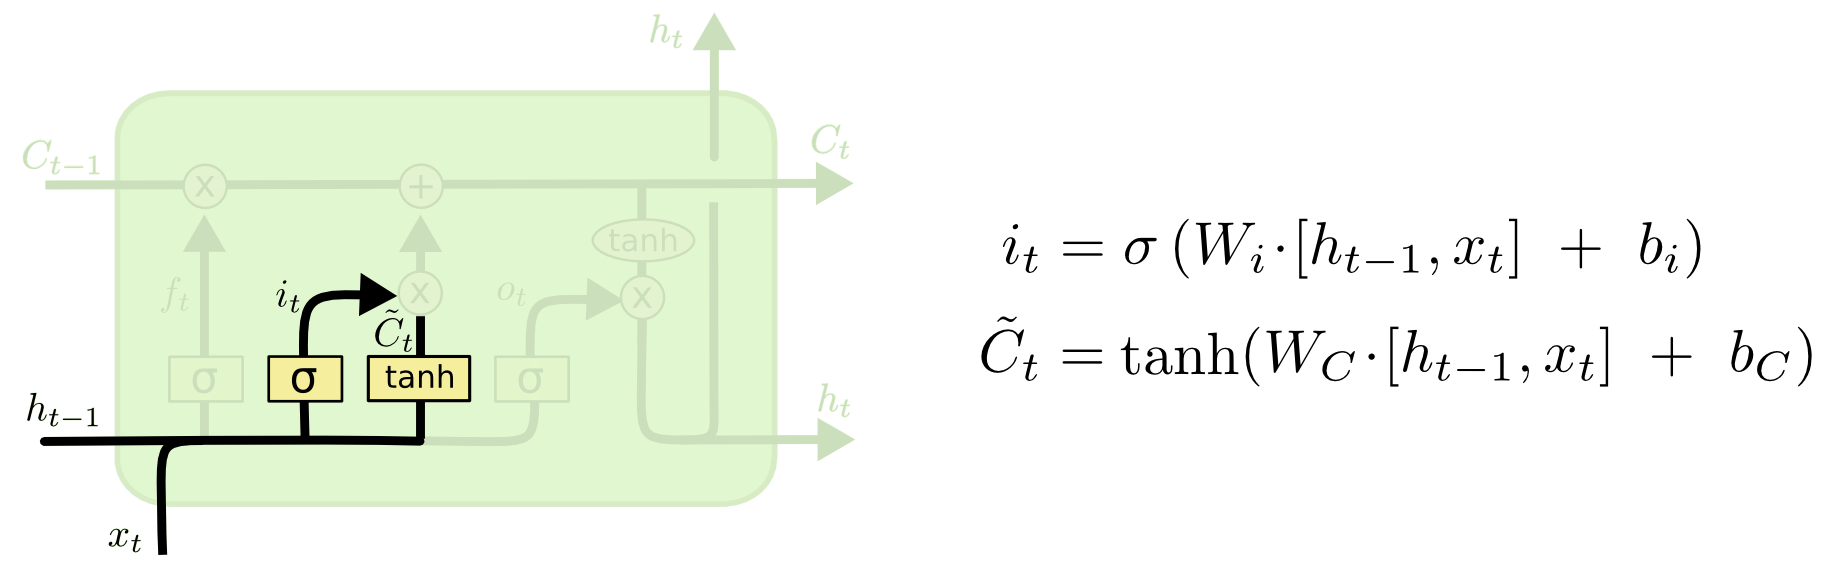
\includegraphics[width=\textwidth]{imagenes/LSTM3-focus-i.png}
	\caption[]{Sección que decide qué valores del vector resumen se actualizarán. (Imagen extraída de \textcite{christopher_olah_2015})}
	\label{fig:lstmAnadir}
\end{figure}


\par En la figura \ref{fig:lstmAnadir} se puede ver como se crean dos vectores uno $\widetilde{C_t}$ y $i_t$ los cuales simbolizan respectivamente los valores candidatos para el resumen y una máscara que filtrará los valores que la red neuronal, después de la retroalimentación, considere importantes. El filtro se aplica cuando se pasa por la unidad que multiplica.

\begin{figure}[H]
	\centering
	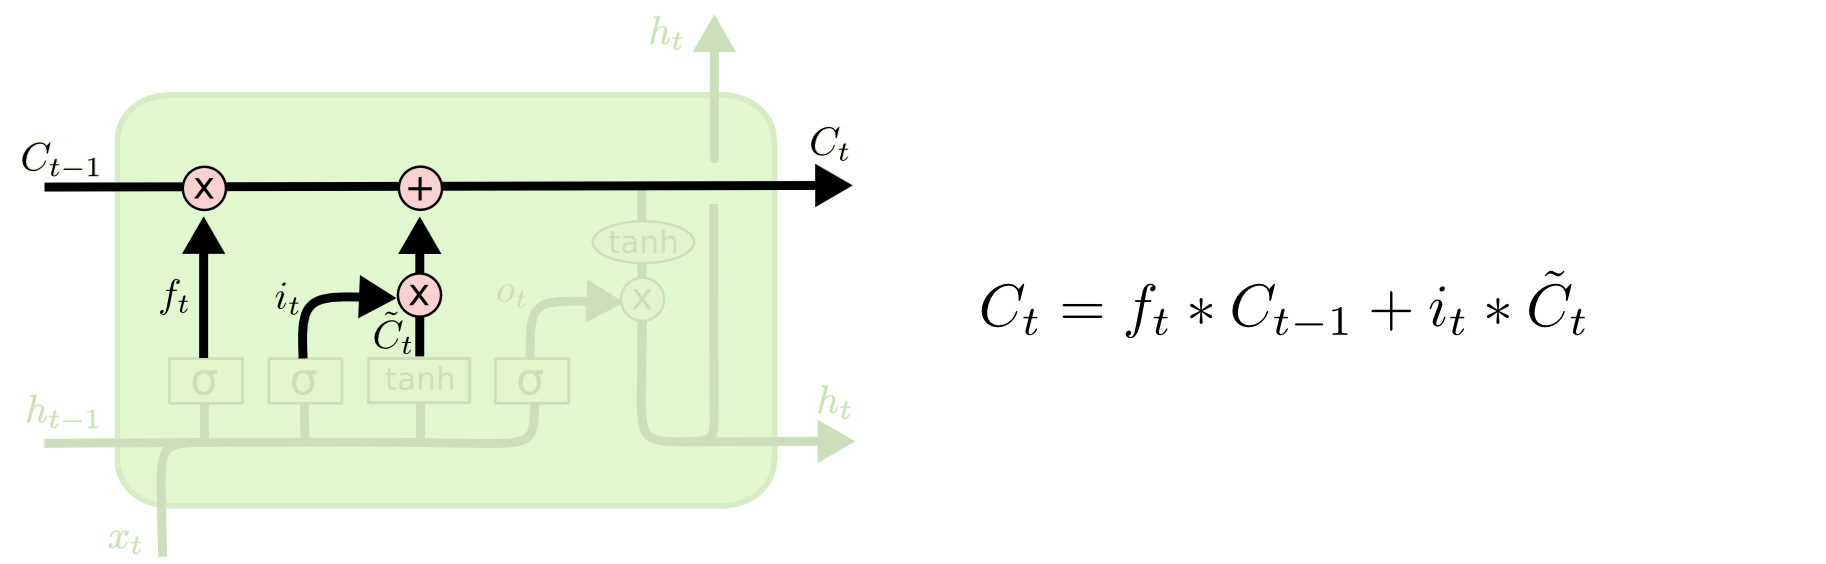
\includegraphics[width=\textwidth]{imagenes/LSTM3-focus-C.png}
	\caption[]{Sección que toma los valores que genera el conocimiento que se añadirá al conocimiento anterior. (Imagen extraída de \textcite{christopher_olah_2015})}
	\label{fig:lstmSuma}
\end{figure}

\par En la figura \ref{fig:lstmSuma} se muestra como las entradas de una unidad cambian para convertirse en la entrada de la siguiente unidad, la unidad para multiplicar tiene el propósito de borrar la memoria de la unidad mientras que la suma tiene el propósito de añadir conocimiento a la siguiente unidad.

\begin{figure}[H]
	\centering
	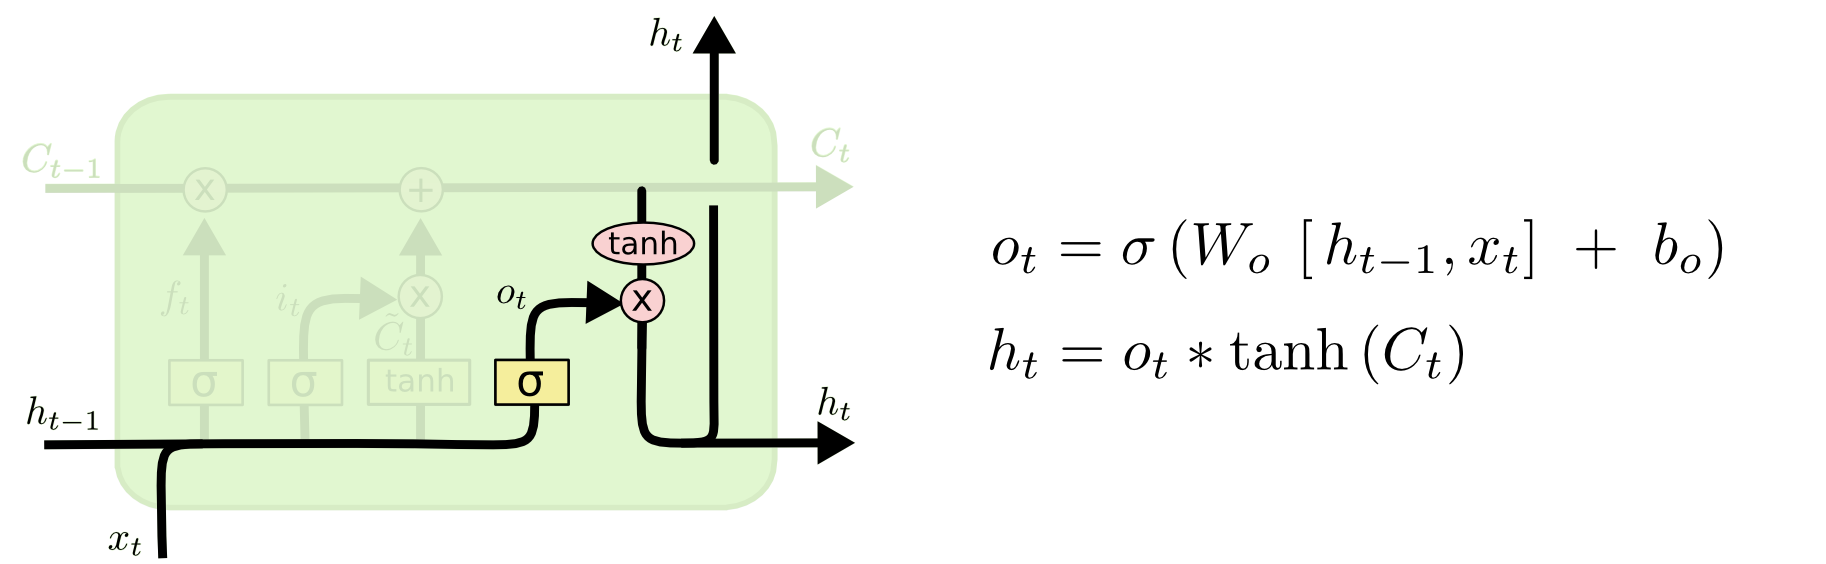
\includegraphics[width=\textwidth]{imagenes/LSTM3-focus-o.png}
	\caption[]{Sección que borra o añade el conocimiento al previo. (Imagen extraída de \textcite{christopher_olah_2015})}
	\label{fig:lstmFinal}
\end{figure}


\par En la figura \ref{fig:lstmFinal} se puede ver que en la unidad se genera la salida actual de la unidad $h_t$ que también es el entrada que recibe la siguiente unidad el cual determinará si la siguiente unidad olvidará o no.

\par Una \gls{bi-lstm} cambia el concepto de LSTM para encontrar la información hacia delante y hacia atrás. Añadiendo una capa que lee hacia atrás, entonces ésta se puede conectar a otra capa de red neuronal (completamente conectada) que los convierte en una salida binaria que decidirá si es irónica o no. En la figura \ref{fig:arquitectura} se puede ver la arquitectura general del sistema.

\begin{landscape}

	\begin{figure}[h]
		\centering
		

\tikzset{every picture/.style={line width=0.75pt}} %set default line width to 0.75pt        

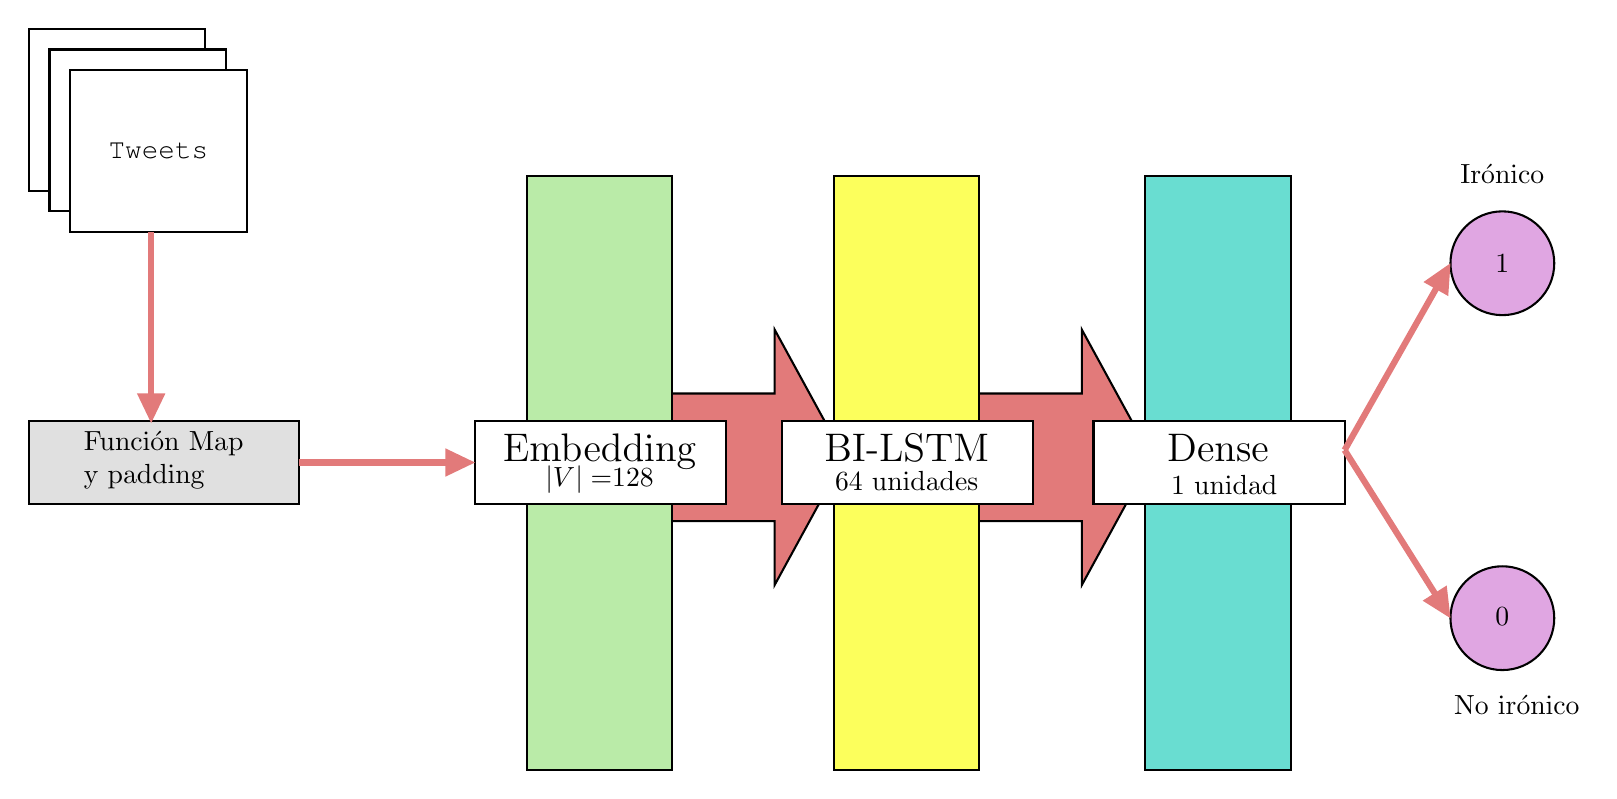
\begin{tikzpicture}[x=0.75pt,y=0.75pt,yscale=-1,xscale=1]
%uncomment if require: \path (0,560); %set diagram left start at 0, and has height of 560

%Right Arrow [id:dp8310111909351754] 
\draw  [fill={rgb, 255:red, 226; green, 122; blue, 122 }  ,fill opacity=1 ] (557,229.75) -- (607.4,229.75) -- (607.4,199) -- (641,260.5) -- (607.4,322) -- (607.4,291.25) -- (557,291.25) -- cycle ;
%Right Arrow [id:dp47914845862025834] 
\draw  [fill={rgb, 255:red, 226; green, 122; blue, 122 }  ,fill opacity=1 ] (409,229.75) -- (459.4,229.75) -- (459.4,199) -- (493,260.5) -- (459.4,322) -- (459.4,291.25) -- (409,291.25) -- cycle ;
%Shape: Rectangle [id:dp6690480869865736] 
\draw  [fill={rgb, 255:red, 186; green, 235; blue, 168 }  ,fill opacity=1 ] (340,125) -- (410,125) -- (410,411) -- (340,411) -- cycle ;
%Shape: Rectangle [id:dp5000001257312081] 
\draw  [fill={rgb, 255:red, 255; green, 255; blue, 255 }  ,fill opacity=1 ] (315,243) -- (436,243) -- (436,283) -- (315,283) -- cycle ;

%Shape: Rectangle [id:dp10129983649453078] 
\draw  [fill={rgb, 255:red, 252; green, 255; blue, 92 }  ,fill opacity=1 ] (488,125) -- (558,125) -- (558,411) -- (488,411) -- cycle ;
%Shape: Rectangle [id:dp5417230650141682] 
\draw  [fill={rgb, 255:red, 255; green, 255; blue, 255 }  ,fill opacity=1 ] (463,243) -- (584,243) -- (584,283) -- (463,283) -- cycle ;

%Shape: Rectangle [id:dp3694545240809384] 
\draw  [fill={rgb, 255:red, 105; green, 221; blue, 209 }  ,fill opacity=1 ] (638,125) -- (708,125) -- (708,411) -- (638,411) -- cycle ;
%Shape: Rectangle [id:dp46595094502729073] 
\draw  [fill={rgb, 255:red, 255; green, 255; blue, 255 }  ,fill opacity=1 ] (613,243) -- (734,243) -- (734,283) -- (613,283) -- cycle ;

%Shape: Rectangle [id:dp8981854115946217] 
\draw  [fill={rgb, 255:red, 255; green, 255; blue, 255 }  ,fill opacity=1 ] (100,54) -- (185,54) -- (185,132) -- (100,132) -- cycle ;
%Shape: Rectangle [id:dp3678809591192025] 
\draw  [fill={rgb, 255:red, 255; green, 255; blue, 255 }  ,fill opacity=1 ] (110,64) -- (195,64) -- (195,142) -- (110,142) -- cycle ;
%Shape: Rectangle [id:dp18627809361061853] 
\draw  [fill={rgb, 255:red, 255; green, 255; blue, 255 }  ,fill opacity=1 ] (120,74) -- (205,74) -- (205,152) -- (120,152) -- cycle ;

%Shape: Rectangle [id:dp5391508691442917] 
\draw  [fill={rgb, 255:red, 224; green, 224; blue, 224 }  ,fill opacity=1 ] (100,243) -- (230,243) -- (230,283) -- (100,283) -- cycle ;

%Straight Lines [id:da3222212402232878] 
\draw [color={rgb, 255:red, 226; green, 122; blue, 122 }  ,draw opacity=1 ][line width=2.25]    (230,263) -- (311,263) ;
\draw [shift={(315,263)}, rotate = 180] [fill={rgb, 255:red, 226; green, 122; blue, 122 }  ,fill opacity=1 ][line width=2.25]  [draw opacity=0] (14.29,-6.86) -- (0,0) -- (14.29,6.86) -- cycle    ;

%Shape: Circle [id:dp5889762673635599] 
\draw  [fill={rgb, 255:red, 224; green, 166; blue, 226 }  ,fill opacity=1 ] (785,167) .. controls (785,153.19) and (796.19,142) .. (810,142) .. controls (823.81,142) and (835,153.19) .. (835,167) .. controls (835,180.81) and (823.81,192) .. (810,192) .. controls (796.19,192) and (785,180.81) .. (785,167) -- cycle ;
%Shape: Circle [id:dp18063293168467354] 
\draw  [fill={rgb, 255:red, 224; green, 166; blue, 226 }  ,fill opacity=1 ] (785,338) .. controls (785,324.19) and (796.19,313) .. (810,313) .. controls (823.81,313) and (835,324.19) .. (835,338) .. controls (835,351.81) and (823.81,363) .. (810,363) .. controls (796.19,363) and (785,351.81) .. (785,338) -- cycle ;
%Straight Lines [id:da9689497769272035] 
\draw [color={rgb, 255:red, 226; green, 122; blue, 122 }  ,draw opacity=1 ][line width=2.25]    (734,257) -- (783.03,170.48) ;
\draw [shift={(785,167)}, rotate = 479.54] [fill={rgb, 255:red, 226; green, 122; blue, 122 }  ,fill opacity=1 ][line width=2.25]  [draw opacity=0] (14.29,-6.86) -- (0,0) -- (14.29,6.86) -- cycle    ;

%Straight Lines [id:da9360660330658093] 
\draw [color={rgb, 255:red, 226; green, 122; blue, 122 }  ,draw opacity=1 ][line width=2.25]    (734,257) -- (782.87,334.62) ;
\draw [shift={(785,338)}, rotate = 237.8] [fill={rgb, 255:red, 226; green, 122; blue, 122 }  ,fill opacity=1 ][line width=2.25]  [draw opacity=0] (14.29,-6.86) -- (0,0) -- (14.29,6.86) -- cycle    ;

%Straight Lines [id:da7770649855526097] 
\draw [color={rgb, 255:red, 226; green, 122; blue, 122 }  ,draw opacity=1 ][line width=2.25]    (159,152) -- (159,240) ;
\draw [shift={(159,244)}, rotate = 270] [fill={rgb, 255:red, 226; green, 122; blue, 122 }  ,fill opacity=1 ][line width=2.25]  [draw opacity=0] (14.29,-6.86) -- (0,0) -- (14.29,6.86) -- cycle    ;


% Text Node
\draw (375,264) node  [align=left] {{\Large Embedding}\\};
% Text Node
\draw (523,264) node  [align=left] {{\Large BI-LSTM}\\};
% Text Node
\draw (673,264) node  [align=left] {{\Large Dense}\\};
% Text Node
\draw (375,271) node  [align=left] {$\displaystyle |V|=$128};
% Text Node
\draw (523,272) node  [align=left] {64 unidades};
% Text Node
\draw (676,274) node  [align=left] {1 unidad};
% Text Node
\draw (162.5,113) node  [align=left] {{\fontfamily{pcr}\selectfont Tweets}};
% Text Node
\draw (165,262) node  [align=left] {Función Map\\y padding};
% Text Node
\draw (810,167) node  [align=left] {1};
% Text Node
\draw (810,337) node  [align=left] {0};
% Text Node
\draw (810,124) node  [align=left] {Irónico};
% Text Node
\draw (817,380) node  [align=left] {No irónico};


\end{tikzpicture}

		\caption{En esta figura se puede ver como es la arquitectura general del modelo que se plantea, primero de los textos extraídos de Twitter se pasan por una función de mapeo que convierte el texto en vectores, estos vectores pueden tener diferentes longitudes, por lo que pasa por un \gls{padding} que regulariza su longitud, después pasa al embedding que tiene como salida vectores de 128 dimensiones, estos a su vez pasan a la capa de BI-LSTM que 64 a su salida un vector de 64 unidades, las cuales pasan a una única neurona con salida binaria, la cual indica si el texto que entró es irónico o no.}
		\label{fig:arquitectura}
	\end{figure}
\end{landscape}



\section{Técnica de evaluación}

\par Una de las partes fundamentales de los modelos de inteligencia es la evaluación, en este proceso se mide de manera cuantitativa como se desempeña un sistema. Para esto existen diferentes métricas para cuantificar este desempeño. Para este experimento se usaron \textit{precisión}, \textit{reclamo} y \textit{valor-F}. Estas métricas dependen directamente de la conocida matriz de confusión, qué se puede observar en la figura \ref{fig:confMat}. 

\begin{figure}[h]
	\centering
	

\tikzset{every picture/.style={line width=0.75pt}} %set default line width to 0.75pt        

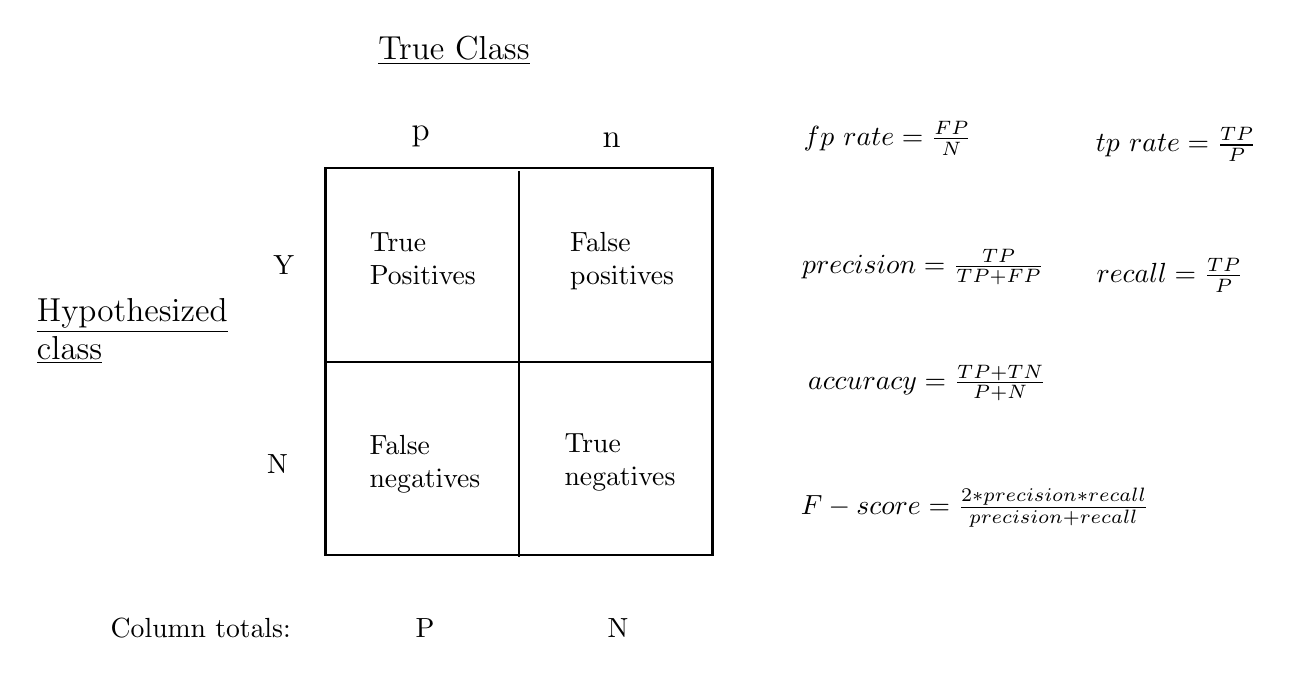
\begin{tikzpicture}[x=0.75pt,y=0.75pt,yscale=-1,xscale=1,thick,scale=1, every node/.style={scale=1}]
%uncomment if require: \path (0,380); %set diagram left start at 0, and has height of 380

%Shape: Square [id:dp7426323050252599] 
\draw   (152.13,94.38) -- (338.5,94.38) -- (338.5,280.75) -- (152.13,280.75) -- cycle ;
%Straight Lines [id:da08397904354123575] 
\draw    (245.31,95.88) -- (245.31,281.92) ;


%Straight Lines [id:da28737204711696407] 
\draw    (152.29,187.56) -- (338.33,187.56) ;





% Text Node
\draw (200,237) node  [align=left] {False\\negatives};
% Text Node
\draw (294,236) node  [align=left] {True\\negatives};
% Text Node
\draw (295,139) node  [align=left] {False\\positives};
% Text Node
\draw (199,138) node  [align=left] {True\\Positives};
% Text Node
\draw (198,79) node  [align=left] {{\large p}};
% Text Node
\draw (290,81) node  [align=left] {{\large n}};
% Text Node
\draw (132,141) node  [align=left] {Y};
% Text Node
\draw (129,237) node  [align=left] {N};
% Text Node
\draw (214,38) node  [align=left] {{\large \underline{True Class}}};
% Text Node
\draw (59,173) node  [align=left] {{\large \underline{Hypothesized}}\\{\large \underline{class}}};
% Text Node
\draw (440,142) node   {$precision=\frac{TP}{TP+FP}$};
% Text Node
\draw (559,146) node   {$recall=\frac{TP}{P}$};
% Text Node
\draw (92,316) node  [align=left] {Column totals:};
% Text Node
\draw (200,316) node  [align=left] {P};
% Text Node
\draw (293,316) node  [align=left] {N};
% Text Node
\draw (423,80) node   {$fp\ rate=\frac{FP}{N}$};
% Text Node
\draw (562,83) node   {$tp\ rate=\frac{TP}{P}$};
% Text Node
\draw (442,198) node   {$accuracy=\frac{TP+TN}{P+N}$};
% Text Node
\draw (465,258) node   {$F-score=\frac{2*precision*recall}{precision+recall}$};


\end{tikzpicture}

	% 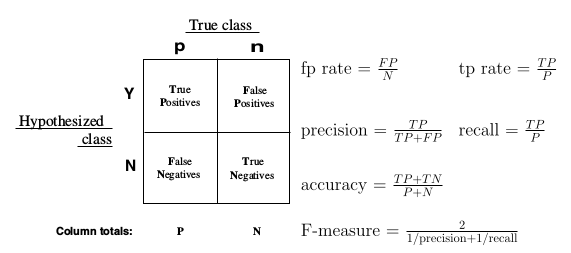
\includegraphics[width=\linewidth]{imagenes/confusionMatrix.png}
	\caption{Matriz de confusión. Imagen extraída de \textcite{fawcett2006introduction}}
	\label{fig:confMat}
\end{figure}

\subsection{Exactitud}

\par La \gls{exactitud} o \textit{accuracy} en inglés, se refiere a una medida de desempeño que se usa para saber que porcentaje de las muestras se predicen correctamente, sin importar de que clase sean. Esta métrica no es idónea para corpus no balanceados, ya que el sistema normalmente va a predecir que todas o la mayoría de las muestras son de una clase. La exactitud puede ser grande aunque no encuentre correctamente las demás clases, sólo con decir que todas las muestras pertenecen a la clase mayoritaria. Su formula es la que se muestra a continuación:
\begin{figure}[H]
	\centering
	\begin{equation*}
		Precision\ =\ \frac{TP+TN}{TP+TN+FN+FP}
	\end{equation*}
	\caption*{TP = verdaderos positivos (muestras que se predicen positivas y que lo son) , FP = falsos positivos (muestras que se predicen negativas y que no lo son), FN =falsos negativos (muestras que se predicen como negativas y que no lo son), TN = verdaderos negativos (muestras que se predicen como negativas y que lo son.)}
\end{figure}

\subsection{Precisión}

\par El \gls{precision} o la \textit{precision} en inglés, se refiere a una medida de desempeño que se usa principalmente en tareas no balanceadas, esta medida trata de reconocer cuantas predicciones positivas fueron correctas entre el total de las respuesta correctas, esto se refiere principalmente a qué tan bien funciona el modelo en detectar las muestras relevantes (en este caso las positivas). La fórmula es la que se muestra a continuación:
\begin{figure}[H]
	\centering
	\begin{equation*}
		Precision\ =\ \frac{TP}{TP+FP}
	\end{equation*}
	\caption*{TP = verdaderos positivos (muestras que se predicen positivas y que lo son) , FP = falsos positivos (muestras que se predicen negativas y que no lo son)}
\end{figure}


\subsection{Reclamo}

\par El \gls{reclamo} o \textit{recall} en inglés se refiere a la medida de desempeño de un modelo que igual que la precisión se usa en tareas con datos no balanceados. Su interpretación índica cual es la porción de muestras que se predicen positivas y lo son, entre el total de las muestras que son positivas, su fórmula es la siguiente:

\begin{figure}[H]
	\centering
	\begin{equation*}
		Recall\ =\ \frac{TP}{P}\ =\ \frac{TP}{TP+FN}
	\end{equation*}
	\caption*{TP = verdaderos positivos (muestras que se predicen positivas y que lo son) , FN = falsos negativos (muestras negativas que se predicen como negativas, pero en realidad son positivos).}
\end{figure}

\subsection{Valor-F}

\par El \gls{valor-F} o \textit{F-Score} en inglés es una medida del desempeño que combina el \textit{recall} y el \textit{precision}, para obtener la media armónica, esto es por que las dos están relacionadas y si una sube la otra baja. Lo importante es tener un equilibrio el cual haría el \textit{f-score} más grande. Una media armónica que trata de no sesgar el resultado de la media al valor más grande sino al mas bajo. La fórmula del f-score es la siguiente:

\begin{figure}[H]
	\centering
	\begin{equation*}
		F-score\ =\ 2 \times  \frac{precision*recall}{precision\ +recall}
	\end{equation*}
\end{figure}

\subsection{Descripción de la forma de evaluación cruzada}

\par Para la forma de evaluación el corpus se subdividió en 5 partes del 20\% cada una, de las cuales se formaron 5 distribuciones del corpus, esto se puede ver mejor en la figura \ref{fig:corpusDiv}.

\begin{figure}[h]
	\centering
	

\tikzset{every picture/.style={line width=0.75pt}} %set default line width to 0.75pt        

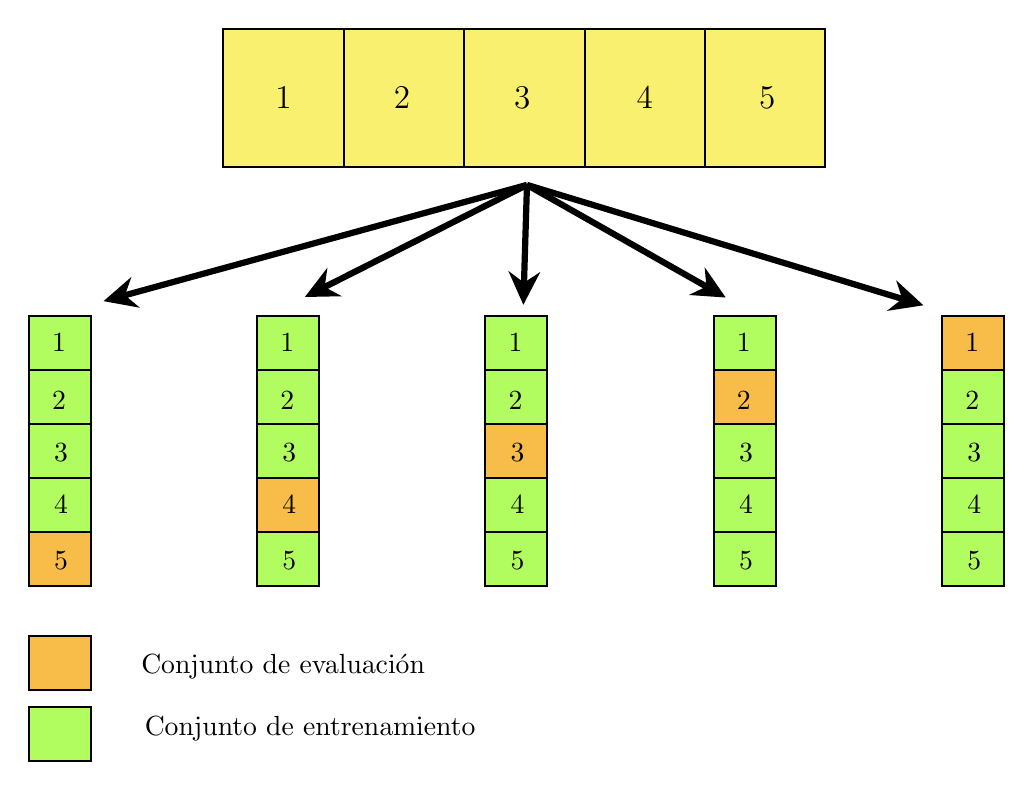
\begin{tikzpicture}[x=0.75pt,y=0.75pt,yscale=-1,xscale=1]
%uncomment if require: \path (0,403); %set diagram left start at 0, and has height of 403

%Shape: Rectangle [id:dp4324979495520729] 
\draw  [fill={rgb, 255:red, 250; green, 240; blue, 111 }  ,fill opacity=1 ] (421.25,41.75) -- (421.25,108.25) -- (363.25,108.25) -- (363.25,41.75) -- cycle ;
%Shape: Rectangle [id:dp4732661957682942] 
\draw  [fill={rgb, 255:red, 250; green, 240; blue, 111 }  ,fill opacity=1 ] (479.25,41.75) -- (479.25,108.25) -- (421.25,108.25) -- (421.25,41.75) -- cycle ;
%Shape: Rectangle [id:dp09264088763089329] 
\draw  [fill={rgb, 255:red, 250; green, 240; blue, 111 }  ,fill opacity=1 ] (363.25,41.75) -- (363.25,108.25) -- (305.25,108.25) -- (305.25,41.75) -- cycle ;
%Shape: Rectangle [id:dp27681985257611963] 
\draw  [fill={rgb, 255:red, 250; green, 240; blue, 111 }  ,fill opacity=1 ] (305.25,41.75) -- (305.25,108.25) -- (247.25,108.25) -- (247.25,41.75) -- cycle ;
%Shape: Rectangle [id:dp35774533585505663] 
\draw  [fill={rgb, 255:red, 250; green, 240; blue, 111 }  ,fill opacity=1 ] (247.25,41.75) -- (247.25,108.25) -- (189.25,108.25) -- (189.25,41.75) -- cycle ;
%Shape: Rectangle [id:dp6300651561593915] 
\draw  [fill={rgb, 255:red, 177; green, 252; blue, 95 }  ,fill opacity=1 ] (125.31,284.39) -- (95.44,284.39) -- (95.44,258.34) -- (125.31,258.34) -- cycle ;
%Shape: Rectangle [id:dp8765465889393704] 
\draw  [fill={rgb, 255:red, 248; green, 189; blue, 72 }  ,fill opacity=1 ] (125.31,310.44) -- (95.44,310.44) -- (95.44,284.39) -- (125.31,284.39) -- cycle ;
%Shape: Rectangle [id:dp27508771757617656] 
\draw  [fill={rgb, 255:red, 177; green, 252; blue, 95 }  ,fill opacity=1 ] (125.31,258.34) -- (95.44,258.34) -- (95.44,232.29) -- (125.31,232.29) -- cycle ;
%Shape: Rectangle [id:dp9828530985786075] 
\draw  [fill={rgb, 255:red, 177; green, 252; blue, 95 }  ,fill opacity=1 ] (125.31,232.29) -- (95.44,232.29) -- (95.44,206.24) -- (125.31,206.24) -- cycle ;
%Shape: Rectangle [id:dp8511798847882142] 
\draw  [fill={rgb, 255:red, 177; green, 252; blue, 95 }  ,fill opacity=1 ] (125.31,206.24) -- (95.44,206.24) -- (95.44,180.19) -- (125.31,180.19) -- cycle ;
%Shape: Rectangle [id:dp24215577820153578] 
\draw  [fill={rgb, 255:red, 248; green, 189; blue, 72 }  ,fill opacity=1 ] (235.31,284.39) -- (205.44,284.39) -- (205.44,258.34) -- (235.31,258.34) -- cycle ;
%Shape: Rectangle [id:dp20025071615226597] 
\draw  [fill={rgb, 255:red, 177; green, 252; blue, 95 }  ,fill opacity=1 ] (235.31,310.44) -- (205.44,310.44) -- (205.44,284.39) -- (235.31,284.39) -- cycle ;
%Shape: Rectangle [id:dp8410616935900397] 
\draw  [fill={rgb, 255:red, 177; green, 252; blue, 95 }  ,fill opacity=1 ] (235.31,258.34) -- (205.44,258.34) -- (205.44,232.29) -- (235.31,232.29) -- cycle ;
%Shape: Rectangle [id:dp9019405855389522] 
\draw  [fill={rgb, 255:red, 177; green, 252; blue, 95 }  ,fill opacity=1 ] (235.31,232.29) -- (205.44,232.29) -- (205.44,206.24) -- (235.31,206.24) -- cycle ;
%Shape: Rectangle [id:dp8723175446401576] 
\draw  [fill={rgb, 255:red, 177; green, 252; blue, 95 }  ,fill opacity=1 ] (235.31,206.24) -- (205.44,206.24) -- (205.44,180.19) -- (235.31,180.19) -- cycle ;
%Shape: Rectangle [id:dp10475735860334345] 
\draw  [fill={rgb, 255:red, 177; green, 252; blue, 95 }  ,fill opacity=1 ] (345.31,284.39) -- (315.44,284.39) -- (315.44,258.34) -- (345.31,258.34) -- cycle ;
%Shape: Rectangle [id:dp8360710594149254] 
\draw  [fill={rgb, 255:red, 177; green, 252; blue, 95 }  ,fill opacity=1 ] (345.31,310.44) -- (315.44,310.44) -- (315.44,284.39) -- (345.31,284.39) -- cycle ;
%Shape: Rectangle [id:dp3251826315662174] 
\draw  [fill={rgb, 255:red, 248; green, 189; blue, 72 }  ,fill opacity=1 ] (345.31,258.34) -- (315.44,258.34) -- (315.44,232.29) -- (345.31,232.29) -- cycle ;
%Shape: Rectangle [id:dp43410729341495813] 
\draw  [fill={rgb, 255:red, 177; green, 252; blue, 95 }  ,fill opacity=1 ] (345.31,232.29) -- (315.44,232.29) -- (315.44,206.24) -- (345.31,206.24) -- cycle ;
%Shape: Rectangle [id:dp2237354541869716] 
\draw  [fill={rgb, 255:red, 177; green, 252; blue, 95 }  ,fill opacity=1 ] (345.31,206.24) -- (315.44,206.24) -- (315.44,180.19) -- (345.31,180.19) -- cycle ;
%Shape: Rectangle [id:dp05371800101329849] 
\draw  [fill={rgb, 255:red, 177; green, 252; blue, 95 }  ,fill opacity=1 ] (455.31,284.39) -- (425.44,284.39) -- (425.44,258.34) -- (455.31,258.34) -- cycle ;
%Shape: Rectangle [id:dp35978328802574344] 
\draw  [fill={rgb, 255:red, 177; green, 252; blue, 95 }  ,fill opacity=1 ] (455.31,310.44) -- (425.44,310.44) -- (425.44,284.39) -- (455.31,284.39) -- cycle ;
%Shape: Rectangle [id:dp11324731127997034] 
\draw  [fill={rgb, 255:red, 177; green, 252; blue, 95 }  ,fill opacity=1 ] (455.31,258.34) -- (425.44,258.34) -- (425.44,232.29) -- (455.31,232.29) -- cycle ;
%Shape: Rectangle [id:dp3713437467654701] 
\draw  [fill={rgb, 255:red, 248; green, 189; blue, 72 }  ,fill opacity=1 ] (455.31,232.29) -- (425.44,232.29) -- (425.44,206.24) -- (455.31,206.24) -- cycle ;
%Shape: Rectangle [id:dp3078959049885366] 
\draw  [fill={rgb, 255:red, 177; green, 252; blue, 95 }  ,fill opacity=1 ] (455.31,206.24) -- (425.44,206.24) -- (425.44,180.19) -- (455.31,180.19) -- cycle ;
%Shape: Rectangle [id:dp9529437202543025] 
\draw  [fill={rgb, 255:red, 177; green, 252; blue, 95 }  ,fill opacity=1 ] (565.31,284.39) -- (535.44,284.39) -- (535.44,258.34) -- (565.31,258.34) -- cycle ;
%Shape: Rectangle [id:dp9922975154494478] 
\draw  [fill={rgb, 255:red, 177; green, 252; blue, 95 }  ,fill opacity=1 ] (565.31,310.44) -- (535.44,310.44) -- (535.44,284.39) -- (565.31,284.39) -- cycle ;
%Shape: Rectangle [id:dp8226822462900152] 
\draw  [fill={rgb, 255:red, 177; green, 252; blue, 95 }  ,fill opacity=1 ] (565.31,258.34) -- (535.44,258.34) -- (535.44,232.29) -- (565.31,232.29) -- cycle ;
%Shape: Rectangle [id:dp6350529855385154] 
\draw  [fill={rgb, 255:red, 177; green, 252; blue, 95 }  ,fill opacity=1 ] (565.31,232.29) -- (535.44,232.29) -- (535.44,206.24) -- (565.31,206.24) -- cycle ;
%Shape: Rectangle [id:dp19244781197245708] 
\draw  [fill={rgb, 255:red, 248; green, 189; blue, 72 }  ,fill opacity=1 ] (565.31,206.24) -- (535.44,206.24) -- (535.44,180.19) -- (565.31,180.19) -- cycle ;
%Straight Lines [id:da9512591343165853] 
\draw [line width=2.25]    (335.5,117) -- (135.36,171.94) ;
\draw [shift={(131.5,173)}, rotate = 344.65] [fill={rgb, 255:red, 0; green, 0; blue, 0 }  ][line width=2.25]  [draw opacity=0] (16.07,-7.72) -- (0,0) -- (16.07,7.72) -- (10.67,0) -- cycle    ;

%Straight Lines [id:da04818720431299961] 
\draw [line width=2.25]    (335.5,117) -- (232.07,169.2) ;
\draw [shift={(228.5,171)}, rotate = 333.22] [fill={rgb, 255:red, 0; green, 0; blue, 0 }  ][line width=2.25]  [draw opacity=0] (16.07,-7.72) -- (0,0) -- (16.07,7.72) -- (10.67,0) -- cycle    ;

%Straight Lines [id:da5826595319338874] 
\draw [line width=2.25]    (335.5,117) -- (333.87,170.75) ;
\draw [shift={(333.75,174.75)}, rotate = 271.74] [fill={rgb, 255:red, 0; green, 0; blue, 0 }  ][line width=2.25]  [draw opacity=0] (16.07,-7.72) -- (0,0) -- (16.07,7.72) -- (10.67,0) -- cycle    ;

%Straight Lines [id:da3687801654619345] 
\draw [line width=2.25]    (335.5,117) -- (522.67,173.84) ;
\draw [shift={(526.5,175)}, rotate = 196.89] [fill={rgb, 255:red, 0; green, 0; blue, 0 }  ][line width=2.25]  [draw opacity=0] (16.07,-7.72) -- (0,0) -- (16.07,7.72) -- (10.67,0) -- cycle    ;

%Straight Lines [id:da5919916039876636] 
\draw [line width=2.25]    (335.5,117) -- (427.77,169.28) ;
\draw [shift={(431.25,171.25)}, rotate = 209.54] [fill={rgb, 255:red, 0; green, 0; blue, 0 }  ][line width=2.25]  [draw opacity=0] (16.07,-7.72) -- (0,0) -- (16.07,7.72) -- (10.67,0) -- cycle    ;

%Shape: Rectangle [id:dp3523228887868648] 
\draw  [fill={rgb, 255:red, 248; green, 189; blue, 72 }  ,fill opacity=1 ] (125.31,360.44) -- (95.44,360.44) -- (95.44,334.39) -- (125.31,334.39) -- cycle ;
%Shape: Rectangle [id:dp08317013348175117] 
\draw  [fill={rgb, 255:red, 177; green, 252; blue, 95 }  ,fill opacity=1 ] (125.31,394.39) -- (95.44,394.39) -- (95.44,368.34) -- (125.31,368.34) -- cycle ;

% Text Node
\draw (218.25,75) node  [align=left] {{\large 1}};
% Text Node
\draw (275.25,75) node  [align=left] {{\large 2}};
% Text Node
\draw (333.25,75) node  [align=left] {{\large 3}};
% Text Node
\draw (392.25,75) node  [align=left] {{\large 4}};
% Text Node
\draw (451.25,75) node  [align=left] {{\large 5}};
% Text Node
\draw (110,193) node  [align=left] {1};
% Text Node
\draw (110,221) node  [align=left] {2};
% Text Node
\draw (111,246) node  [align=left] {3};
% Text Node
\draw (111,271) node  [align=left] {4};
% Text Node
\draw (111,298) node  [align=left] {5};
% Text Node
\draw (220,193) node  [align=left] {1};
% Text Node
\draw (220,221) node  [align=left] {2};
% Text Node
\draw (221,246) node  [align=left] {3};
% Text Node
\draw (221,271) node  [align=left] {4};
% Text Node
\draw (221,298) node  [align=left] {5};
% Text Node
\draw (330,193) node  [align=left] {1};
% Text Node
\draw (330,221) node  [align=left] {2};
% Text Node
\draw (331,246) node  [align=left] {3};
% Text Node
\draw (331,271) node  [align=left] {4};
% Text Node
\draw (331,298) node  [align=left] {5};
% Text Node
\draw (440,193) node  [align=left] {1};
% Text Node
\draw (440,221) node  [align=left] {2};
% Text Node
\draw (441,246) node  [align=left] {3};
% Text Node
\draw (441,271) node  [align=left] {4};
% Text Node
\draw (441,298) node  [align=left] {5};
% Text Node
\draw (550,193) node  [align=left] {1};
% Text Node
\draw (550,221) node  [align=left] {2};
% Text Node
\draw (551,246) node  [align=left] {3};
% Text Node
\draw (551,271) node  [align=left] {4};
% Text Node
\draw (551,298) node  [align=left] {5};
% Text Node
\draw (218,349) node  [align=left] {Conjunto de evaluación};
% Text Node
\draw (231,379) node  [align=left] {Conjunto de entrenamiento};


\end{tikzpicture}

	\caption{Del corpus total se separaron 5 versiones las cuales cambian su sección de prueba y de entrenamiento, para después promediar sus puntajes.}
	\label{fig:corpusDiv}
\end{figure}

\par Sobre estos 5 grupos se entrenó el mismo clasificador usando el 80\% para entrenamiento y el 20\% para la fase de evaluación. Los datos que se ven en el capítulo \ref{cap.experimentos} se promedian y se reportan.

\subsection{ROC y AUC}

\par Otra forma de evaluación que se realizará es la métrica ROC y AUC. Una gráfica \textit{`receiver operating characteristics (ROC)'} es un método gráfico para calificar el desempeño de un clasificador.
\par En este caso consistirá desplazar el umbral de discretización para observar cómo se da el aumento de los \textit{true positive rate} y \textit{false positive rate}. Esta gráfica es bastante sencilla, sin embargo, su interpretación no es nada trivial, por lo que no se tratará a fondo en esta tesis.

\par Esta métrica ayuda a visualizar fácilmente qué pasa con el comportamiento de un clasificador cuando se le cambia el umbral. Para entenderla se debe analizar una curva ROC muestra.

\begin{figure}[H]
	\centering
	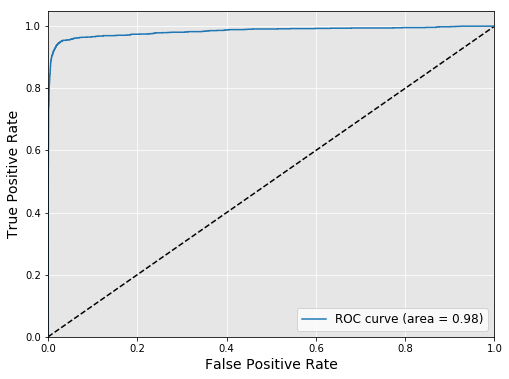
\includegraphics[width=0.8\linewidth]{imagenes/ROC_Exp3_1.png}
	\caption{Curva ROC experimento 3}
	\label{fig:ROCMuestra}
\end{figure}

\par En la figura \ref{fig:ROCMuestra} se puede observar una recta a \ang{45} la cual es la recta que se obtendría si se hace una clasificación aleatoria. Luego la recta azul es la recta que se obtuvo de mover el umbral de 0 a 1. Se puede ver que cuando el umbral es 0, todas las muestras serán positivas entonces el \textit{false positive rate} y el  \textit{true positive rate} aumentarán a 1 o lo que es lo mismo se tendrá un punto en (1,1). Por el lado contrario si se tiene el umbral en 1 el \textit{false positive rate} y el  \textit{true positive rate} disminuirán a 0 y se tendrá un punto en (0,0). Lo que se busca con este modelo es tener el \textit{true positive rate} en 1 y el \textit{false positive rate} en 0 o lo que es lo mismo tener un punto en (0,1). Como es muy probable que el modelo tenga dicho punto, se puede considerar que entre más cerca mejor y esto se logra si se tienen bien separadas las clases. Es decir, cuando se tiene una clase en un extremo del umbral y la otra del otro, de este modo, el movimiento del umbral no afectará tanto en la clasificación. Esto es lo que mide la gráfica ROC.

\par Para hablar del \textit{area under the curve} es la reducción de la gráfica ROC a un escalar el cual es representado por el área bajo la curva, esto indica qué tanto se pudo acercar al punto deseado (0,1) y qué tan estable es el modelo al clasificar.

\subsection{Justificación}

\par El \textit{recall} y el \textit{precision} son las medidas que generalmente se usan para medir el desempeño, principalmente porque aportan información sobre qué tan bien realizan la tarea cuando los datos no están balanceados, lo cual sucede la mayoría de las veces. Además el \textit{f-score} aporta una mejor utilidad ya que aporta información de ambas medidas, sin tender a sesgar el resultado por el valor más grande sino por el más pequeño.

\par La gráfica ROC y el AUC son métodos gráficos ampliamente utilizados que pueden servir para rápidamente identificar si un modelo tiene un buen desempeño o no, por lo que se considera valioso para los experimentos.


